
%%%%%%%%%%%%%%%%%%%%%%%%%%%%%%%%
%------------------------------%
%%%%%%%%%%%%%%%%%%%%%%%%%%%%%%%%
\section{\anna{Introduction}}
%%%%%%%%%%%%%%%%%%%%%%%%%%%%%%%%
%------------------------------%
%%%%%%%%%%%%%%%%%%%%%%%%%%%%%%%%
Genetic association studies have become increasingly widespread in recent years, due to their success in identifying thousands of genetic variants associated with diseases and complex traits. Accurately identifying and estimating the effect sizes of these variants or single nucleotide polymorphisms (SNPs) is of interest for a variety of scientific applications. This information can be used to predict an individual's risk of disease, elucidate the genetic architecture underlying a complex trait, and guide drug discovery. Genome-wide association studies (GWAS) are the most common method of analyzing genetic data sets, and involve independently testing each variant. However, this approach can fail to identify true associations due to the high significance thresholds required to account for multiple comparisons.

An additional hurdle such analyses must contend with is that of population structure such as population stratification or cryptic relatedness. The presence of such structure can adversely affect analyses in several ways. Firstly, allele frequency differences due to ancestry within a sample can be mistaken for biological signal if steps are not taken to mitigate this effect. One common solution, chopping up a sample and performing ancestry-specific analyses, often results in a loss of statistical power from reduced sample sizes. Secondly, correlation among subjects within a sample, whether due to common ancestry or more recent relatedness, violates the independent errors assumption that many regression methods rely on, rendering statistical methods such as linear and logistic invalid.

Additionally, testing one SNP at a time may not account for linkage disequilibrium (LD), or correlation among loci. Consequently, signals of association may be mis-attributed to SNPs in the absence of true biological association. One commonly used method for analyzing data in the presence of correlated loci is LD pruning, which involves sequentially thinning SNPs that exceed a correlation threshold, so that only variants that are relatively independent are used in modeling and testing procedures. An alternative solution is the use of multivariate methods such as multiple linear regression, which adjusts for and estimates the effects of numerous variants simultaneously. However, classical multivariate approaches rely on data with more observations than unknown parameters. This is typically infeasible in genome-wide studies where the number of variants greatly exceeds the number of individuals. 

Penalized regression methods make such problems tractable by constraining the solution space of coefficient estimates. The lasso is a widely used penalized regression method \citep{tibshirani1996regression}.  It relies on an assumption of sparsity; in other words, that many features will have no effect. Thus, although the total number of features may be large, the number that actually affect the outcome will be small. This allows coefficient estimation and variable selection to be accomplished simultaneously, and provides considerable computational advantages that scale up well to very large data sets. These features make the lasso attractive for the analysis of high-dimensional genetic data where identifying the variants most highly associated with a particular trait is often of interest. Although separately testing each SNP is still the most common way of analyzing GWAS data, the use of lasso and related methods is increasing in use due to computational advances that make it practical to apply on a genome-wide scale \citep{qian2020fast, prive2018efficient}. 

As with multiple linear regression models, lasso penalized regression assumes independent observations and uncorrelated errors. In the presence of population structure or cryptic relatedness, however, samples are correlated, violating this assumption. If unaccounted for, this dependency can result in the identification of spurious associations. Though methods to correct for population stratification and cryptic relatedness have been extensively investigated, the majority of this work has focused on plant and animal breeding data, a setting which affords much greater experimental control than studies of human genetics \citep{Amin2007, hoffman2013correcting, price2006principal, rakitsch2013lasso, bhatnagar2020simultaneous, Sillanpaeae2011}. While many standard correction techniques may in principle be applied to human genetic data, their performance has not been well-studied within the context of human ancestry and confounding arising from observational study \citep{lawson2019population, barton2019population}.  

One reason that population stratification warrants such concern in genetic studies is that due to ethnic and geographic segregation, population stratification tends to be associated with differing environmental exposures and cultural practices \citep{thornton2015statistical, browning2011population}. In other words, random genetic variation is likely to be correlated with non-genetic factors that also influence the trait of interest, thereby confounding the genotype-phenotype relationship and leading to spurious associations and biased estimates of SNP effects. Biased estimates of this nature severely hinder prediction and understanding differences among populations \citep{barton2019population}. Although bias at individual loci may be small, this bias becomes magnified when aggregated across thousands of SNPs, as is done when calculating polygenic risk scores \citep{barton2019population, peterson2019genome}.

In order to clarify and emphasize the importance of the subtle distinction between population structure and environmental heterogeneity, we present a detailed review of relevant concepts and methods. The remainder of this paper is organized as follows. In Section \ref{sec:background} we provide a summary of the causes and consequences of structure in the genetic data of seemingly unrelated individuals and formally define terminology used throughout this work. We emphasize that confounding due to population structure, frequently cited as a driver of spurious associations, is a function of environmental heterogeneity, where genetic data serves as a proxy for differential environmental exposures \citep{Sillanpaeae2011, sul2018population, vilhjalmsson2012nature, barton2019population}. In so doing, we refine the definition of confounding due to population structure in terms of a non-genetic mechanism. In addition, we briefly review historical methods of correcting for population stratification and relatedness. In Section \ref{sec:methods} we provide a detailed review of the two most prevalent multivariate methods of adjusting for population stratification and relatedness at present: PCA adjusted lasso penalized regression (PC-lasso) and lasso penalized multivariate LMMs (LMM-lasso). We review the statistical details of how these methods attempt to correct for population structure and environmental heterogeneity. In Section \ref{sec:results}, we illustrate these concepts via simulation studies, where the data-generating mechanism allows us to distinguish between population structure and environmental heterogeneity. In addition, these results identify scenarios where particular methods may be most and least effective in accurately estimating the effect sizes of observed SNPs in the presence of unobserved confounding.

%%%%%%%%%%%%%%%%%%%%%%%%%%%%%%%%
%------------------------------%
%%%%%%%%%%%%%%%%%%%%%%%%%%%%%%%%
\section{Background} \label{sec:background}
%%%%%%%%%%%%%%%%%%%%%%%%%%%%%%%%
%------------------------------%
%%%%%%%%%%%%%%%%%%%%%%%%%%%%%%%%

%------------------------------%
\subsection{Structure in genetic data}

Population structure is defined by the existence of allele frequency differences that distinguish subpopulations and is driven by the combined effects of evolutionary processes such as genetic drift, migration, demographic history, and natural selection \citep{gibson2015primer, tibayrenc2017genetics}. Population structure is broadly categorized based on whether it describes recent or ancient relatedness. Ancient relatedness describes the presence of a common ancestor many generations previously. The presence of distinct ancestry groups with different allele frequencies in a sample is known as \textbf{population stratification}. Recent relatedness describes the sharing of a common ancestor only a few generations previous. Pedigree-based methods may be used to explicitly model recent relatedness if familial relationships are known. In the absence of known familial relationships, recent relatedness is referred to as \textbf{cryptic relatedness.} 

Population structure is a common phenomenon in genetic data. Varying levels of relatedness are almost always present among genetic samples, even in those of unrelated individuals and seemingly homogeneous populations. For example, European American, Han Chinese, and most recently, cohorts within the UK Biobank data have been shown to exhibit patterns of population and geographic structure despite their seemingly similar subjects \citep{campbell2005demonstrating, xu2009genomic, chen2009genetic, haworth2019apparent}.

In this review we focus on methods to account for unobserved dependence between samples, whether arising from population stratification or cryptic relatedness. Throughout this paper, the terms \textbf{population structure} and \textbf{structured population} will be used to describe a sample of individuals in which population stratification, cryptic relatedness, or both are present. Population stratification in particular has been of great concern in genetic studies due to its potential to lead to spurious associations when population structure is associated with differences in both allele frequency and the trait or disease of interest \citep{gibson2015primer}. This phenomenon is commonly described as \textbf{confounding due to population stratification}. The mechanism of this phenomenon warrants some discussion as it is often overlooked that population structure in and of itself does not confound the genotype-phenotype relationship. Rather, there must also exist some non-genetic mechanism by which population stratification affects the phenotype, namely, the environment \citep{barton2019population, vilhjalmsson2012nature}.


%------------------------------%
\subsection{Motivating example} \label{sec:example}

As an example, consider a genome wide association study (GWAS) to assess genetic variants associated with lung cancer in a sample comprised of subjects from two distinct subpopulations, A and B. Assume the minor allele of SNP $X$ is more common in subpopulation B compared to subpopulation A, but has no direct effect on lung cancer. Also suppose these subpopulations are geographically segregated in a such a way that subpopulation A is exposed to good air quality, and subpopulation B to poor air quality, and that air quality does have a direct effect on lung cancer. A GWAS of data from these subpopulations would likely find SNP $X$ to be significantly associated with lung cancer. This spurious association is does not arise from the presence of population stratification itself, but because that stratification is related to a causal environmental exposure. Indeed, if subpopulations A and B were not subject to different air qualities, all else being equal, SNP $X$ would not be associated with the phenotype.

This mechanism of environmental confounding is summarized in the directed acyclic graph displayed in diagram \eqref{diag:ps_env}. The undirected dashed line between population stratification and environmental exposure indicates that while we assume these elements are correlated, we do not assume any causal direction.
%Otherwise stated, we do not assume that environmental factors directly influence population-specific allele frequencies, or vice versa, only that the two may be related.
In the context of our air quality example, this means that we assume air quality is not directly altering individuals' allele frequencies, nor are allele frequencies causing individuals to move to regions of better or worse air quality, only that they are now correlated. Genetic relatedness and environmental effects may become associated over time for any number of complex reasons beyond the scope of this paper. However, as we will discuss, many methods of correcting for population structure rely on this relationship and do not formally differentiate between effects of population structure and those of environment. Such methods assume that genetic relatedness serves as an accurate proxy for environmental exposures, which may or may not be the case depending on the exposure and population in question.

\begin{equation}
\centering
\begin{tikzpicture}[baseline=(current  bounding  box.center)]
    \node (1) at (0,0) {Population Stratification};
    \node (2) [right = of 1] {Environment};
    \node (3) [below = of 1] {Observed SNPs};
    \node (4) [below = of 2] {Phenotype};
    \path[bidirected, -] (1) edge (2);
    \path (1) edge (3);
    \path (2) edge (4);
    \path (3) edge (4);
\end{tikzpicture}
\label{diag:ps_env}
\end{equation}

%\begin{equation}
%\centering
%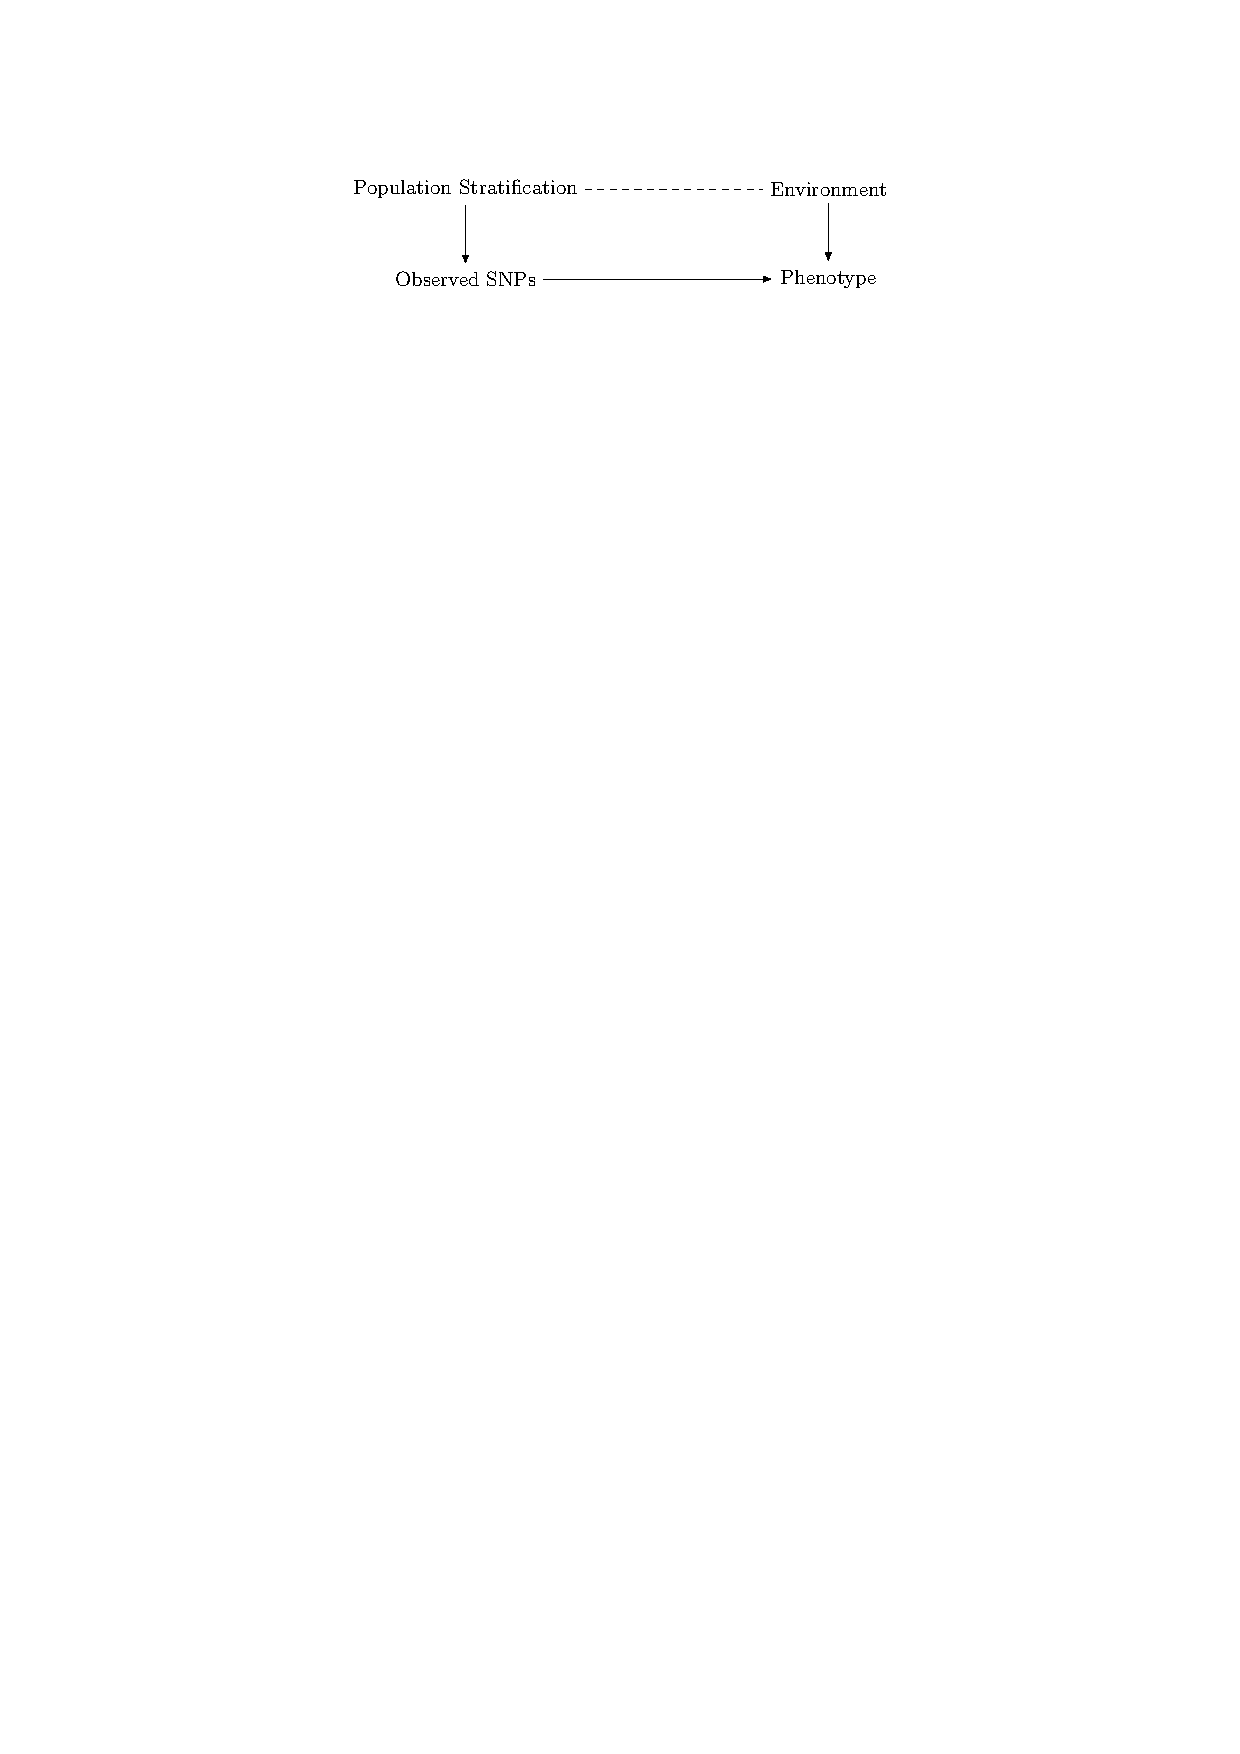
\includegraphics{figures/dag1.png}
%\label{diag:ps_env}
%\end{equation}

A different type of confounding in genetic studies that we will briefly mention is due to genetic background. This occurs in univariate association methods when a non-causal SNP is tested for association with a trait of interest, and that SNP is correlated with a causal SNP. As \citet{vilhjalmsson2012nature} note, any trait that has some genetic basis will be subject to genetic background effects, just as traits that are influenced by the environment may be subject to environmental confounding. Given the importance of both genetic and environmental contributions to many complex phenotypes, both genetic background and environmental confounding are important factors in our ability to identify true causal genetic relationships between SNPs and phenotype. As mentioned earlier, LD pruning is a common approach to reduce confounding due to genetic background in univariate association testing. Here, we focus on methods which address this via genomewide multivariate analysis.

%------------------------------%
\subsection{Correcting for population structure}
\label{Sec:correcting-structure}

One of the earliest approaches to address the problem of confounding due to population structure was the method of genomic control (GC). Because confounding inflates the distribution of association test statistics, GC introduces a factor to counteract this effect and restore the appropriate null distribution. This deflation factor is estimated using loci independent of the phenotype of interest and the loci being tested for association \citep{devlin1999genomic, bacanu2000power, wang2009testing}. However, quantifying the extent of inflation is not trivial, and is sensitive to the nature and quantity of the loci used to estimate it \citep{hellwege2017population, marchini2004effects}. Additionally, GC does not correct effect size estimates, so resulting coefficient estimates will be unreliable after GC is applied, even if their corresponding test statistics and p-values have been appropriately adjusted \citep{hellwege2017population}.

New statistical methods to control for the effects of confounding due to population stratification have proliferated as computational advances have allowed for the analysis of genetic data from large cohorts. Many of these methods attempt to block the causal pathway between population structure and observed SNP data. This is illustrated by the blocked arrow in diagram \eqref{diag:ps_env_block}. As the figure shows, these methods do not directly address the environmental component of confounding due to population structure, instead controlling confounding by indirectly blocking the causal pathway between the environment and observed SNPs. 

\begin{equation}
\centering
\begin{tikzpicture}[baseline=(current  bounding  box.center)]
    \node (1) at (0,0) {Population Stratification};
    \node (2) [right = of 1] {Environment};
    \node (3) [below = of 1] {Observed SNPs};
    \node (4) [below = of 2] {Phenotype};
    \path[bidirected, -] (1) edge (2);
    \path[line width = 0.5] (1) edge (3);
    \path (2) edge (4);
    \path (3) edge (4);
    \tkzMarkSegment[pos=.5,mark=x](1,3)
\end{tikzpicture}
\label{diag:ps_env_block}
\end{equation}

%Whether or not such methods are effective at reducing confounding effects depends upon whether population structure can be accurately inferred.
As mentioned earlier, population structure only leads to confounding if it is correlated with a causal effect in the environment.
In the presence of environmental heterogeneity which affects the phenotype of interest in a manner that is orthogonal to population structure, SNP-phenotype associations will not be confounded. This is due to the absence of a causal pathway between population stratification and environment, as depicted in diagram \eqref{diag:ps_env_block2}. In such a scenario, failing to account for unobserved environmental effects is likely to result in greater variability, but SNP effect estimates will remain unbiased \citep{greenland1999causal}. We will discuss this fact in greater detail in Section \ref{sec:partition}.

\begin{equation}
\centering
\begin{tikzpicture}[baseline=(current  bounding  box.center)]
    \node (1) at (0,0) {Population Stratification};
    \node (2) [right = of 1] {Environment};
    \node (3) [below = of 1] {Observed SNPs};
    \node (4) [below = of 2] {Phenotype};
    \path[bidirected, -] (1) edge (2);
    \path (1) edge (3);
    \path (2) edge (4);
    \path (3) edge (4);
    \tkzMarkSegment[pos=.5,mark=x](1,2)
\end{tikzpicture}
%\caption{The causal pathway between the environment and observed SNPs may be blocked if genetic information does not serve as an accurate proxy for it.}
\label{diag:ps_env_block2}
\end{equation}

Assuming for now that population structure is correlated with environmental exposures and can be accurately inferred from available data, we return to our consideration of methods that attempt to control for confounding via the mechanism depicted in diagram \eqref{diag:ps_env_block}. Such methods include LMMs, principal-component-based approaches, and structured association. Structured, or stratified, association refers to a general class of methods which attempt to infer subject membership within a discrete number of nonoverlapping subpopulations. The analysis is conducted within each subpopulation, and the subpopulation-specific results may then be combined via meta-analysis \citep{pritchard1999use, pritchard2000association}. By partitioning the overall sample size in this manner, the structured association method is vulnerable to a loss of power. Additionally, it relies on the assumption that these subpopulations are distinct and nonoveralapping. This assumption may not accurately reflect the characteristics of a particular sample, such as one consisting of admixed populations, or recent relatedness. Considered in the context of our air quality example, rather than the existence of two subpopulations with exposure to either good or bad air quality, we may have a continuous gradient of relatedness and air quality. By clustering individuals into one subpopulation or another, we oversimplify the population structure.

A different approach is to use create surrogate variables to represent population structure, and to adjust for these as additional model covariates. Principal component-adjustment (PC-adjustment) methods use the first several eigenvectors a pairwise similarity matrix as these surrogate variables \citep{price2006principal}. This approach may be used in univariate or multivariate frameworks, and allows for analysis on the entirety of a structured sample. 

The term LMM has been used to describe a number of distinct but related procedures for analyzing structured genetic data which differ in their objectives and methods. There are two main objectives of LMMs in the genetics context: estimating narrow-sense heritability, and estimating individual SNP effects.

Among LMM methods that aim to estimate heritability, the most well-known is genome-wide complex trait analysis (GCTA) \citep{yang2011gcta}. In this framework, all observed SNPs are treated as random effects. These effects are integrated out in order to estimate a genetic variance component, which in turn, is used to quantify the total narrow-sense heritability of a trait \citep{yang2010common}.

LMMs can also be used to estimate SNP effects, and this can be done in either a univariate or multivariate manner. Like PC-adjustment methods, LMMs utilize a similarity matrix to estimate and subsequently correct for relatedness among subjects. In an LMM, however, the surrogate variables are treated as random, rather than fixed effects \citep{yu2006unified, kang2010variance, kang2008efficient}. However, as with all univariate testing approaches, univariate LMM implementations are subject to spurious associations and biased effect estimates in the presence of LD. 

Multivariate mixed model approaches reduce these problems by modeling the relationship between a phenotype of interest and all SNPs simultaneously via penalized regression, while correcting for dependencies among subjects \citep{rakitsch2013lasso, bhatnagar2020simultaneous}. This approach assumes there are a relatively small number of SNPs associated with the phenotype of interest that have large effect sizes. These SNPs will be included in the model as both fixed and random effects, while SNPs with smaller effect sizes are modeled only as part of the random effect in order to control for dependent errors due to relatedness and sample structure. 

\anna{In many genetic association studies the phenotype of interest is binary, for example the presence or absence of a heritable trait. However, the extension of LMMs and penalized LMMs to nonlinear models is not straightforward. LMMs and penalized LMMs are able to efficiently correct for dependencies among subjects by preprocessing the data by means of a weighted rotation. This procedure does not generalize beyond the linear regression case where the outcome is continuous. Because of this, distinct inferential algorithms are required to extend the LMM modeling methodology to nonlinear models such as logistic regression. \citet{mandt2017sparse} generalize the LMM modeling paradigm to binary phenotypes in the interest of classification. They do so by thresholding the outcome variable through a Probit likelihood with additional sparsity constraints and approximate Bayesian inference. However, to the best of our knowledge, the joint problem of sparse estimation in the presence of dependent observations has been limited to the linear regression case \citep{seeger2011large, vattikuti2014applying, rakitsch2013lasso}.}

The remainder of this review will focus on the performance of such multivariate lasso-penalized methods for the analysis of continuous, normally distributed outcomes. Specifically, PC-adjustment and LMM methods, which we will refer to as PC-lasso and LMM-lasso, respectively. We consider two similar implementations of the LMM-lasso method, one developed by \citet{rakitsch2013lasso} and a more recent implementation from \citet{bhatnagar2020simultaneous}. Subsequent references to LMM-lasso apply to both implementations, unless otherwise stated. Where necessary, we will differentiate between these implementations by referring to them as LMM-lasso-Rakitsch and LMM-lasso-ggmix, respectively. 

Several studies have shown that LMMs outperform PC-adjustment methods in the univariate framework \citep{wang2013analytical, kang2010variance, zhao2007arabidopsis}. However, to the best of our knowledge this is the only comprehensive review and comparison of these methods in a penalized multivariate framework and using a simulation scheme motivated by human genetics and environmental confounding.\\

%%%%%%%%%%%%%%%%%%%%%%%%%%%%%%%%
%------------------------------%
%%%%%%%%%%%%%%%%%%%%%%%%%%%%%%%%
\section{Methods} \label{sec:methods}
%%%%%%%%%%%%%%%%%%%%%%%%%%%%%%%%
%------------------------------%
%%%%%%%%%%%%%%%%%%%%%%%%%%%%%%%%
%------------------------------%
\subsection{\anna{lasso}}
\anna{not sure if you/reviewers were thinking more lasso background should go here vs. somewhere else. I initially tried to add more background to the introduction but didn't think additional information "fit" there given what was already there. I'm open to having additional lasso background elsewhere though.}
We begin by briefly reviewing the key methodological components of the lasso. In the usual linear regression set-up where there is a continuous response $\by \in \real^n$, an $n \times p$ design matrix $\bX$, and a parameter vector $\bbeta \in \real^p$, the ordinary lasso minimizes the objective function

\begin{equation}
    Q(\bbeta | \lam) = \frac{1}{2n}|| \by -  \beta_0 - \bX \bbeta ||_2^2 + \lam ||\bbeta||_1,
\end{equation}
where $|| \boldsymbol{\beta} ||_1 = \sum_{j=1}^p |\beta_j|$ denotes the $\ell_1$ norm of the regression coefficients, and $||\mathbf{x}||_2 = \sqrt{\sum_{i=1}^p x_i^2}$ the $\ell_2$ norm. The first component of the objective function is the linear regression loss function, which quantifies the overall model fit and captures how well the estimated parameters agree with the observed data. The second component is the $\ell_1$ penalty applied to the estimated coefficient values (but not the intercept, $\beta_0$), which discourages large, unrealistic parameter values. The tuning parameter, $\lambda$, controls the tradeoff between these two components. For sufficiently large values of $\lambda$ all elements of $\bbeta$ will be estimated to be 0. In the $p \ll n$ setting, if $\lam = 0$, the lasso solution coincides with that of ordinary least squares (OLS). The lasso assumes observations are independent. However, the $\ell_1$ penalty of the lasso can also be applied to nonlinear models such as Cox regression \citep{tibshirani1997lasso} and logistic regression \citep{shevade2003simple} by replacing the residual sum of squares with the appropriate negative log-likelihood function.


%------------------------------%
\subsection{LMM and PC models}
\label{Sec:lmm-and-pc}

To describe and compare PC-lasso and LMM-lasso, we consider an $n \times p$ matrix of genotype data $\bG$ for $n$ subjects and $p$ SNPs, where each $G_{ij} \in \{ 0, 1, 2 \}$ enumerates the number of allele copies subject $i$ has for SNP $j$. In order to equitably compare SNP effects across differing allele frequencies, in practice $\bG$ is standardized; not doing so introduces a bias in which common SNPs are more likely to be selected. We denote the standardized version of this genotype matrix as $\bX$, where each $X_{ij} = (G_{ij} - 2 \pi_j) / \sqrt{2\pi_j (1 - \pi_j)}$ and $\pi_j$ is the minor allele frequency (MAF) of SNP $j$ \citep{zhang2015principal, price2006principal}. Additionally, $\bX_0$ represents an $n \times p_0$ matrix of unpenalized covariates and the intercept. At a minimum, $\bX_0$ will be an $n \times 1$ vector of 1s to represent the intercept, in which case $\bbeta_0 \equiv \beta_0$ is the scalar intercept. However, $\bX_0$ may additionally include observed covariates such as age, sex, or smoking history, which are included in the model without penalty. We assume that the $n \times 1$ vector of continuous phenotype values, $\by$, can be expressed as the sum of these covariates, additive SNP effects, environmental effects, and observational noise, and consider the linear model,
\begin{equation}
    \label{eqn:model}
    \by = \bX_0 \bbeta_0 + \bX\bbeta + \bZ\bgamma + \beps
\end{equation}
where $\bbeta_0$ is a $p_0 \times 1$ vector which includes the intercept term and the effects of any unpenalized covariates, $\bbeta$ is a $p \times 1$ vector of SNP effects, $\bgamma$ is a $q \times 1$ vector of environmental effects, $\bZ$ is an $n \times q$ matrix that allocates environmental effects among subjects, and $\beps \sim N(\boldsymbol{0}, \sigmaee \bI_n)$. Often it is assumed that subjects belong to $q \le p$ subpopulations, and $\bZ$ is a corresponding incidence matrix of 0s and 1s. However, this is not the only possibility.

A key feature which differentiates \eqref{eqn:model} from traditional linear mixed models is that in our setting, $\bZ$ is not observed directly, although we still wish to correct for it in order to remove the effects of confounding influences. A common convention is to assume $\bZ = \bX$ \citep{wang2018multiplex, lippert2011fast, yang2014advantages}; we will discuss the rationale for this approach in Section~\ref{sec:partition}.  This, in turn, motivates the methods by which LMM-lasso and PC-lasso attempt to model unobserved confounding effects using observed genetic data.

Both PC-lasso and LMM-lasso rely on matrix decompositions of $\bX$ and the realized relationship matrix (RRM), $\bK = p^{-1} \bX \bX^\T$, which describes the pair-wise genetic similarity among subjects \citep{patterson2006population, hayes2009increased}. Using the singular value decomposition (SVD) of the standardized genotype matrix, we can derive the spectral decomposition of the RRM: 
\begin{equation}
    \label{eqn:k}
    \bK = \frac{1}{p} \bX \bX^\T = \frac{1}{p} \bU \bD^2 \bU^\T = \frac{1}{p} \bR \bR^\T,
\end{equation}
where $\bR = \bU\bD$ and $\bD^2$ is an $n \times n$ diagonal matrix containing the $k$ nonzero eigenvalues of $\bK$ on the top-left diagonal, followed by $n - k$ zeroes. $\bU$ is the corresponding $n \times n$ orthonormal matrix of eigenvectors of $\bK$. The first $k$ columns of $\bU$ correspond to the nonzero eigenvalues of $\bK$, and the columns of $\bR$ are thus the principal components of $\bK$ weighted by their corresponding singular values. 

%------------------------------%
\subsection{PC-lasso}
PC-lasso uses the first $k$ principal components of $\bK$ to approximate $\bZ\bgamma$ and includes them in the model as unpenalized covariates. This corresponds to the regression model
\begin{equation}
    \label{eqn:pca_reg}
    \by = \bX_0\bbeta_0 + \bX\bbeta + \bU_{1:k}\boldsymbol{\alpha} + \beps 
\end{equation}
$$ \beps \sim N(\boldsymbol{0}, \sigmaee \bI), $$
where $\bU_{1:k}$ is the $n \times k$ matrix of principal component vectors, $\boldsymbol{\alpha}$ a corresponding $k \times 1$ coefficient vector, and all other parameters are as defined in equation \eqref{eqn:model}. In a penalized regression framework, this model yields the objective function
\begin{equation}
    \label{eqn:pca_obj}
    Q(\bbeta, \boldsymbol{\alpha}|\bX, \by) = \frac{1}{2n} ||\by - \bX_0\bbeta_0 - \bX \bbeta- \bU_{1:k}\boldsymbol{\alpha}||_2^2 + \lambda || \bbeta ||_1,
\end{equation}
where the principal component regression coefficients, $\boldsymbol{\alpha}$, are not included in the penalty term. 

%------------------------------%
\subsection{LMM-lasso}
\label{sec:lmmlasso}

Conversely, LMM-lasso models $\bZ\bgamma$ as a random effect, which corresponds to the LMM model
\begin{equation}
  \begin{aligned}
    \label{eqn:lmm_reg}
    \by &= \bX_0\bbeta_0 + \bX\bbeta + \bX\bgamma+ \beps, \\
    \beps &\sim N(\boldsymbol{0}, \sigmaee \bI) \\
 \bgamma &\sim N(\boldsymbol{0}, p^{-1} \sigmass \bI) \Rightarrow \bX \bgamma \sim N(\boldsymbol{0}, \sigmass \bK),
  \end{aligned}
\end{equation}
where $\sigmass$ determines the size of the structured component to the variance, and we assume $\beps \independent \bgamma$. Rather than assuming anything about $\bgamma$ directly, a common representation parameterizes the model in terms of $\bu=\bX\bgamma$, which yields an equivalent model. 

We will first derive the LMM-lasso objective function in the absence of unpenalized covariates for the sake of simplicity. Following equation \eqref{eqn:lmm_reg}, in the absence of unpenalized covariates the LMM assumes $\by \sim N(\bX \bbeta, \bV)$, where $\bV = \sigmass \textbf{K} + \sigmaee \textbf{I}$. LMM-lasso uses the covariance structure of the errors and properties of the multivariate normal distribution to transform the original data and diagonalize the errors in a manner akin to generalized least squares (GLS). Specifically, left-multiplying the original data by $\bV^{-1/2}$ yields 

\begin{equation}
\label{eqn:rtY_distn}
\bV^{-\frac{1}{2}}\by \sim N(\bV^{-\frac{1}{2}} \bX \bbeta, \bI),
\end{equation}
and thus an ordinary lasso model can be fit on the transformed data, ($\bV^{-\frac{1}{2}}\bX, \bV^{-\frac{1}{2}}\by$). 

Using the decomposition of $\bK$ described in equation \eqref{eqn:k}, we can gain further insight into the mechanism of this transformation. Note that $\bV^{-1}$ can be expressed using the following matrix factorization 
\begin{align*}
    \bV^{-1} &= (\sigmass \bK + \sigmaee \bI)^{-1}\\
    &=(\sigmass \bU \bD^2 \bU^\T + \sigmaee \bU \bU^\T)^{-1}\\
    &= (\bU (\sigmass \bD^2 + \sigmaee \bI) \bU^\T)^{-1}\\
    &=\bU (\sigmass \bD^2 + \sigmaee \bI)^{-1} \bU^\T\\
    &=\bU \bW^2 \bU^\T.
\end{align*}
By incorporating these decompositions, the transformed data can be expressed as $\bW \bXT$ and $\bW \byT$, respectively, where $\bXT = \bU^\T \bX$, $\byT = \bU^\T \by$, $\bW = \text{diag}\{w_1, ... w_n\}$, and $w_i$ corresponds to the square root of the $i$th element of the diagonal matrix $(\sigmass \bD^2 + \sigmaee \bI)^{-1}$. Together, this yields the objective function
\begin{equation}
\label{eqn:lmm_obj}
Q(\bbeta | \bXT, \byT, \bW) = || \bW (\byT - \bXT \bbeta)||_2^2 + \lambda || \bbeta ||_1.
\end{equation}
In the presence of an intercept and unpenalized covariates, \eqref{eqn:rtY_distn} becomes 
\begin{equation}
\bV^{-\frac{1}{2}}\by \sim N\left(\bV^{-\frac{1}{2}} \bX{^\prime} \bbeta{^\prime}, \bI \right),
\end{equation}
where $\bX{^\prime} = \begin{bmatrix} \bX_0 & \bX \end{bmatrix}$ and $\bbeta{^\prime} = \begin{bmatrix} \bbeta_0^\T & \bbeta^\T \end{bmatrix}^\T$. This in turn leads the objective function
\begin{equation}
Q(\bbeta | \bXT{^\prime}, \byT, \bW) = || \bW (\byT - \bXT{^\prime} \bbeta{^\prime})||_2^2 + \lambda || \bbeta ||_1,
\end{equation}
where $\bXT{^\prime} = \bU^\T \bX{^\prime}$, so that all of the data are transformed, but only the elements of $\bbeta{^\prime}$ corresponding to SNPs are penalized. 

%------------------------------%

Different variance component estimation methods lead to different estimates of $\bW$ and two distinct LMM-lasso variants: LMM-lasso-Rakitsch and LMM-lasso-ggmix. LMM-lasso-Rakitsch uses a two-step procedure for estimating the variance components, $\sigmaee$ and $\delta := \sigmaee / \sigmass$ \citep{rakitsch2013lasso}. These variance components and the corresponding weights are estimated once under the assumption of a null model. A lasso model can then be fit on the transformed data to estimate $\boldsymbol{\beta}$ using standard software for coordinate descent, such as \texttt{glmnet} \citep{glmnet} or \texttt{ncvreg} \citep{ncvreg}. LMM-lasso-ggmix iteratively updates $\widehat{\boldsymbol{\beta}}$ and the variance components via a block coordinate descent algorithm \citep{bhatnagar2020simultaneous}. This iterative update scheme prevents the use of standard lasso software, but is implemented in the \texttt{R} package \texttt{ggmix}. \anna{Should we still reference glmnet, ncvreg, ggmix here if we now include a software section?} We further discuss differences between these methods in Section \ref{sec:results}.

%------------------------------%
\subsection{Relationship between PC-lasso and LMM-lasso}

It has been shown that the random effect formulation of model \eqref{eqn:model} used by LMM-lasso can be equivalently expressed in terms of fixed effects, in the absence of penalization. \citet{zhang2015principal} derived this equivalence using a probabilistic PCA formulation, while \citet{hoffman2013correcting} used the singular value decomposition of $\bX$, which we briefly review.

Using the result of the decomposition from \eqref{eqn:k}, $\bK = p^{-1} \bR \bR^\T$ , the LMM model \eqref{eqn:lmm_reg} can be written equivalently as
\begin{equation}
  \begin{aligned}
    \label{eqn:pc_lmm_equiv}
    \by &= \bX_0 \bbeta_0 + \bX \bbeta + \bR \bgamma + \beps \\
    \beps &\sim N(\boldsymbol{0}, \sigmaee \bI) \\
    \bgamma &\sim N(\boldsymbol{0}, p^{-1} \sigmass \bI) \Rightarrow \bR \bgamma \sim N(\boldsymbol{0}, \sigmass \bK).
  \end{aligned}
\end{equation}
Based on the relationship between equations \eqref{eqn:pca_reg} and \eqref{eqn:pc_lmm_equiv}, we can see that modeling the principal components of $\bK$ as fixed or random effects relies on the same underlying regression model. However, while the LMM includes all the principal components, only $k < n$ are included in the fixed effects model. 

Additionally, while the fixed effects model considers the principal components of $\bK$, the LMM considers the principal components weighted by their corresponding eigenvalues. The eigenvalues have been shown to serve as a measure of biological relevance of each principal component in relation to underlying population structure \citep{hoffman2013correcting, price2006principal}. 

From a Bayesian perspective, using the first $k$ principal components as regression covariates can be viewed as assigning uniform priors to the first $k$ components of $\bgamma$, while the remaining $n - k$ components receive a prior with unit mass at zero. These assignments imply certainty that the effect of population structure on the phenotype is fully captured by the first $k$ PCs. In contrast, the LMM approach can be viewed as assigning a Gaussian prior on each component of $\bgamma$, with variances proportional to the corresponding eigenvalues \citep{astle2009population}. 



Whether modeled as a fixed or random effect, the underlying effect of $\bZ \bgamma$ on phenotype remains the same, but its treatment as a fixed or random effect has important implications in terms of model fitting and estimation. Modeling unobserved confounding using fixed effects requires estimation of $p_0 + p + k$ parameters, compared to the $p_0 + p + 2$ required of an LMM, which may result in a loss of power \citep{zhang2015principal}. Additionally, when modeling $\bZ \bgamma$ using fixed effects, determining the appropriate number of principal components, $k$, to adjust for is non-trivial, and has been the subject of numerous studies \citep{patterson2006population, zhao2018practical}. It has been shown that including too many or too few principal components can result in power loss or increased Type I errors, respectively \citep{zhang2015principal}. Nevertheless, a common practice is to include the ten largest principal components in the analysis \citep{zhao2018practical}. This is the approach we take when implementing PC-lasso in Section \ref{sec:results}.

%------------------------------%
\subsection{Partitioning the effects of environmental confounding}
\label{sec:partition}

In Section~\ref{Sec:correcting-structure}, we remarked that population structure only leads to confounding if it is correlated with the
environment, and in Section~\ref{Sec:lmm-and-pc}, we remarked that in LMM modeling, a typical albeit somewhat mysterious assumption is that $\bZ=\bX$.  Here, we provide explicit mathematical justifications for those statements.  In doing so, we derive a partitioning relationship that illustrates how LMMs achieve bias reduction due to environmental confounding.

We begin by noting that in the GWAS context, the $\bgamma$ term in \eqref{eqn:model} is a fixed effect, although treated as ``random'' in the linear mixed model.  This is done because the confounding environmental effects are unobserved; by considering them to be random, we can integrate over their unknown effects and obtain a marginal likelihood.  However, in terms of a repeated sampling perspective, they are fixed.  If repeated samples were drawn from the same populations, the confounding environmental effects would remain the same, not randomly change from sample to sample.  

Consider our earlier example, where $\bgamma$ represented the effect of air quality.  Clearly, a GWAS that failed to account for population stratification would tend to identify as risk factors SNPs that were simply more common in the population with poor air quality.  Treating $\bgamma$ as random, however, would mean that in one sample, a given population is exposed to good air quality, while in the next, it may be exposed to bad air quality.  Any theoretical or numerical investigation of statistical properties would therefore fail to reveal any bias in this situation, as the two situations would cancel out.

To illustrate this concept mathematically, consider the OLS estimates of $\bbeta$ based on model \eqref{eqn:lmm_reg} where, without loss of generality, we assume $\bX_0 \bbeta_0 = \boldsymbol{0}$ for the sake of simplicity: 
\begin{align}
    \mathbb{E}(\bbetaHat) &= (\bX^\T \bX)^{-1} \bX^\T \mathbb{E}(\by) \notag \\
    &=  (\bX^\T \bX)^{-1} \bX^\T \mathbb{E}(\bX\bbeta + \bX\bgamma + \beps) \label{eqn:expectation}\\
    &\quad \notag\\
    \mathbb{V}(\bbetaHat) &= (\bX^\T \bX)^{-1} \bX^\T \mathbb{V}(\by) \bX  (\bX^\T \bX)^{-1} \notag\\
    &=  (\bX^\T \bX)^{-1} \bX^\T \mathbb{V}(\bX\bbeta + \bX\bgamma + \beps) \bX  (\bX^\T \bX)^{-1} \notag\\
    &=  (\bX^\T \bX)^{-1} \bX^\T \mathbb{V}(\bX\bgamma + \beps) \bX  (\bX^\T \bX)^{-1} \label{eqn:variance}.
\end{align}
Treating the environmental effects as random with $\bgamma \sim N(\boldsymbol{0}, p^{-1} \sigmass \bI)$, equations \eqref{eqn:expectation} and \eqref{eqn:variance} yield $\mathbb{E}(\bbetaHat) = \bbeta$, and $\mathbb{V}(\bbetaHat) = p^{-1}\sigmass\bI + \sigmaee (\bX^\T \bX)^{-1}$, respectively. Treating them as fixed, on the other hand, we have $\mathbb{E}(\bbetaHat) = \bbeta + \bgamma$ and $\mathbb{V}(\bbetaHat) = \sigmaee (\bX^\T \bX)^{-1}$. Treating $\bgamma$ as random gives the misleading impression that the unadjusted association between SNP and phenotype is unbiased.

Let us then decompose the environmental effects $\bZ \bgamma$ into two parts: a component that can be projected onto the column space of $\bX$ and a component that cannot. Let $\P_{\bX} = \bX (\bX^\T \bX)^{-1} \bX^\T$ denote the projection matrix of $\bX$, with $\mathcal{C}(\P_{\bX})$ and $\mathcal{N}(\P_{\bX})$ denoting the column and null spaces of $\P_{\bX}$, respectively. Then there exist $\boldsymbol{\tau}, \boldsymbol{\psi}$ such that $\bZ \bgamma = \bX \boldsymbol{\tau + \psi}$, where $\bX \boldsymbol{\tau} \in \mathcal{C}(\P_{\bX})$ and $\boldsymbol{\psi} \in \mathcal{N}(\P_{\bX})$.  This in turn means that
\begin{equation}
  \begin{aligned}
    \label{eqn:partition_e}
    \by &= \bX\bbeta + \bZ\bgamma + \beps \\
    &= \bX\bbeta + \bX \boldsymbol{\tau} + \boldsymbol{\psi} + \beps \\
    &=  \bX \bbeta{^*} + \beps{^*},
  \end{aligned}
\end{equation}
where $\bbeta^* = \bbeta + \boldsymbol{\tau}$ and $\beps{^*} = \boldsymbol{\psi} + \beps$.  Note that $\boldsymbol{\tau}$ quantifies bias in the na\"ive estimate $\bbetaHat^*$ and $\boldsymbol{\psi}$ is absorbed by the residual error term. In other words, any model specified in terms of $\bZ$ and $\bgamma$ is equivalent to a parameterization using $\bX$ and $\boldsymbol{\tau}$.  This result provides the explicit mathematical justification for the statement in Section~\ref{sec:background} that population structure only biases the SNP-phenotype association if it is correlated with the environmental effects (in the sense that $\bZ\bgamma$ can be projected onto the column space of $\bX$). It furthermore illustrates why the assumption $\bZ=\bX$ in the linear mixed model is reasonable, as well as how it works to remove bias in estimation.

Finally, it is worth noting that the proportion of environmental effects in the column space of $\P_{\bX}$ (i.e., the portion that will cause confounding) is given by
\begin{equation}
    \label{eqn:ratio}
    \text{CP} = ||\bX \boldsymbol{\tau}||_2^2 / ||\bZ \bgamma||_2^2,
\end{equation}
which we refer to as the Confounding Proportion (CP). The CP can range from 0 (no confounding) to 1. In the extreme case where $\bZ \bgamma$ is completely independent of population structure, $\bZ \bgamma \in \mathcal{N}(\P_{\bX})$ and $\bX \boldsymbol{\tau} = \boldsymbol{0}$ so that $\mathbb{E}(\bbetaHat^*) = \bbeta$. In this scenario, the SNP-phenotype associations will be unbiased, although the residual error will be inflated. 

In real data settings CP cannot be calculated since $\bZ \bgamma$ is not directly observed. In simulation settings, however, this ratio is a useful metric for quantifying the degree to which $\bZ \bgamma$ reflects population structure and has the potential to bias observed associations. We use CP to help interpret the simulation results in Section \ref{sec:results}. %In high dimensions, we use a low-rank approximation of $(\bX^\T \bX)^{-1}$ to improve stability.

%------------------------------%
\subsection{Simulation study}
%------------------------------%

\subsubsection{Synthetic phenotypes}

Given the nature of environmental confounding in our setting of interest, we simulate from
\begin{equation}
    \label{eqn:sim}
    \by = a \bX \bbeta + b \bZ \bgamma + c \beps,
\end{equation}
where $\by$ represents the synthetic phenotype, $\bgamma$ is a fixed quantity (see Section~\ref{sec:partition}), and $a, b, c$ are scaling factors. These factors are determined such that the variance of $\by$ is equal to 1 and can be partitioned into genetic signal, environmental confounding, and random noise components, respectively, as follows:
\begin{equation}
    \label{eqn:parition_y}
    \mathbb{V}(\by) = \eta + (1 - \eta) \xi + (1-\eta)(1-\xi).
\end{equation}
In \eqref{eqn:parition_y}, $\eta$ defines the proportion of the variance of $\by$ attributable to additive genetic factors, commonly referred to as the narrow-sense heritability. %, $h^2 = \sigmass/(\sigmass + \sigmaee)$. 
The parameter $\eta$ also describes the data-generating model's signal to noise ratio (SNR), while $\xi$ partitions the remaining variance of $\by$ into latent environmental heterogeneity and random noise. So, for example $\eta = 0.5$ and $\xi = 0.8$ corresponds to a 1:1 SNR, and means that 50\% of the variability in $\by$ is due to additive genetic effects, 40\% due to unobserved environmental effects, and the remaining 10\% due to other factors.

\subsubsection{Genotypes}
\label{sec:subpopulation_structure}

We generated three varieties of genotype matrices $\bG$, which were then standardized to yield the corresponding $\bX$ matrix: (1) simulated SNP data from admixed subpopulations \citep{Ochoa2016}, (2) simulated SNP data from independent subpopulations \citep{Ochoa2016}, and (3) real genome-wide SNP data from known Caucasian ($n = 417$), African American ($n = 134$), and Hispanic ($n = 37$) subpopulations \citep{larkin2015objectives}. We refer to these as 1D Linear Admixture, Independent Subpopulations, and Empirical, respectively. For all data types, there are $p = 1000$ total SNPs, 50 of which have causal effects. For the simulated 1D Linear Admixture and Independent Subpopulations data $n = 200$ unless otherwise specified, and $n = 588$ for the Empirical data. 

For the fully simulated data, two subpopulation structures were considered, which we refer to as ``fine'' and ``coarse''.  We define a coarse structure to be one characterized by a few large subpopulations intended to model large-scale environmental heterogeneity and population stratification, such as that described in our motivating air quality example. Conversely, we define a fine structure to be one characterized by many small subpopulations, representing a continuum of environmental heterogeneity. Whether fine or coarse, the simulated data were generated such that subpopulations (also known as founding populations) are of equal size. We note that the distinction between fine and coarse structure is an entirely different concept than the level of admixture in the simulated data. It is the size of the subpopulations, not the level of admixture, that determines what we refer to as fine or coarse structure. For example, both the Independent Subpopulation and 1D Linear Admixture simulated data may be comprised of fine or coarse structure. However, the subpopulations will be more distinct in the Independent Subpopulation data than in the 1D Linear Admixed data. The Empirical data is comprised of three racial subpopulations; one relatively large, one small, and one in the middle. Thus it represents a hybrid of our simulated coarse and fine structures, with little apparent admixture. Supplementary Figures \ref{fig:admixed} - \ref{fig:empirical} illustrate the simulated kinship structures, as well as that for the Empirical SNP data. 

\subsubsection{Patterns of environmental effects}

In our simulations, $\bZ$ is a matrix of indicator functions identifying subpopulation (founding population) membership, which assigns the corresponding environmental effect $\bgamma$. Various $\bgamma$ patterns were considered in order to investigate the effects of distinct patterns of environmental confounding.  Simulations were carried out with dichotomous (high/low) environmental effects, as well as more complex heterogeneous effects of all different sizes.  In addition, we examined the ``concordance'' of the environmental effect: whether individuals in genetically similar subpopulations experience similar environmental effects or not.  In our experiments, however, neither the heterogeneity nor the concordance of the environmental effects had any meaningful impact on the performance of the methods under consideration.  Thus, throughout Section~\ref{sec:results}, we present results only for discordant, dichotomous environmental effects, as the other results are very similar.

\subsubsection{Tuning parameter selection}

Selection of the tuning parameter $\lambda$ plays an important role in all penalized regression methods, with many possible approaches. Here, for each model, we selected the $\lam$ value such that 50 SNPs were selected (recall that 50 is also the true number of causal SNPs). This method for selecting $\lambda$ was chosen in an attempt to compare the performance of all methods fairly, and as a strategy to evaluate methods in terms of variable selection, as it allows for direct comparison of the first 50 variables each method lets into the model.

Although cross-validation (CV) and information criterion-based methods are commonly used to select $\lambda$ values, in this context they have the potential to result in misleading comparisons. Because lasso, PC-lasso, and LMM-lasso use different likelihoods, an information-criterion-based approach such as BIC would not lend itself to comparable results across methods. Meanwhile, whether cross-validation is advisable or not in the presence of dependent samples is an open question \citep{roberts2017cross}. \anna{We include a more detailed discussion of tuning parameter selection methods for penalized LMMs in Section \ref{sec:discussion}.}


%------------------------------%
\subsection{\anna{Genomewide analysis}}
%------------------------------%

%------------------------------%
\subsection{\anna{Software}}
%------------------------------%
\label{sec:software}

All analyses and simulations were performed using \texttt{R} version 3.6.3. The ordinary lasso and PC-lasso methods were implemented using \texttt{glmnet} \citep{glmnet}. As described previously, LMM-lasso-ggmix was implemented using \texttt{ggmix} \citep{bhatnagar2020simultaneous}. The LMM-lasso-Rakitsch method was implemented using the \texttt{R} package, \texttt{penalizedLMM}, available on the github repository \url{https://github.com/areisett/penalizedLMM}. Although \citet{rakitsch2013lasso} parameterize their model in terms of the variance components $\sigmass$ and $\delta := \sigmaee / \sigmass$, \texttt{penalizedLMM} implements the LMM-lasso-Rakitsch method using an equivalent but more interpretable parameterization in terms of $\eta$ and $\sigmaee$. \texttt{penalizedLMM} additionally implements the elastic net, and the nonconvex penalties, MCP and SCAD.  


%%%%%%%%%%%%%%%%%%%%%%%%%%%%%%%%
%------------------------------%
%%%%%%%%%%%%%%%%%%%%%%%%%%%%%%%%
\section{Results} \label{sec:results}
%%%%%%%%%%%%%%%%%%%%%%%%%%%%%%%%
%------------------------------%
%%%%%%%%%%%%%%%%%%%%%%%%%%%%%%%%

%------------------------------%
\subsection{PC-lasso and LMM-lasso increase accuracy}
\label{sec:sim-mse}
%------------------------------%

We begin by comparing the ordinary lasso, PC-lasso, and LMM-lasso as the level of environmental confounding is varied. Estimation accuracy for lasso, PC-lasso, and LMM-lasso was evaluated based on mean squared error (MSE) of the coefficients, MSE = $\mathbb{E}||\bbeta - \bbetaHat(\lambda)||^2_2$, where $\bbetaHat(\lambda)$ is the vector of coefficients estimated by the lasso with a penalty of $\lambda$, and $\bbeta$ the true coefficient values.
Figure \ref{fig:mse} presents these results for all three data types in a 1:1 SNR setting, where $\eta = 0.5$. The top row of Figure \ref{fig:mse} shows that when $\xi = 0$ (i.e., no environmental effects), lasso and LMM-lasso perform comparably. PC-lasso results in a slight inflation in MSE compared to the other methods in the simulated data sets due to the fact that 10 additional predictors (PCs) have been added to the model, but none of them actually explain any variability in the outcome. 

\begin{figure}[H]
    \centering
    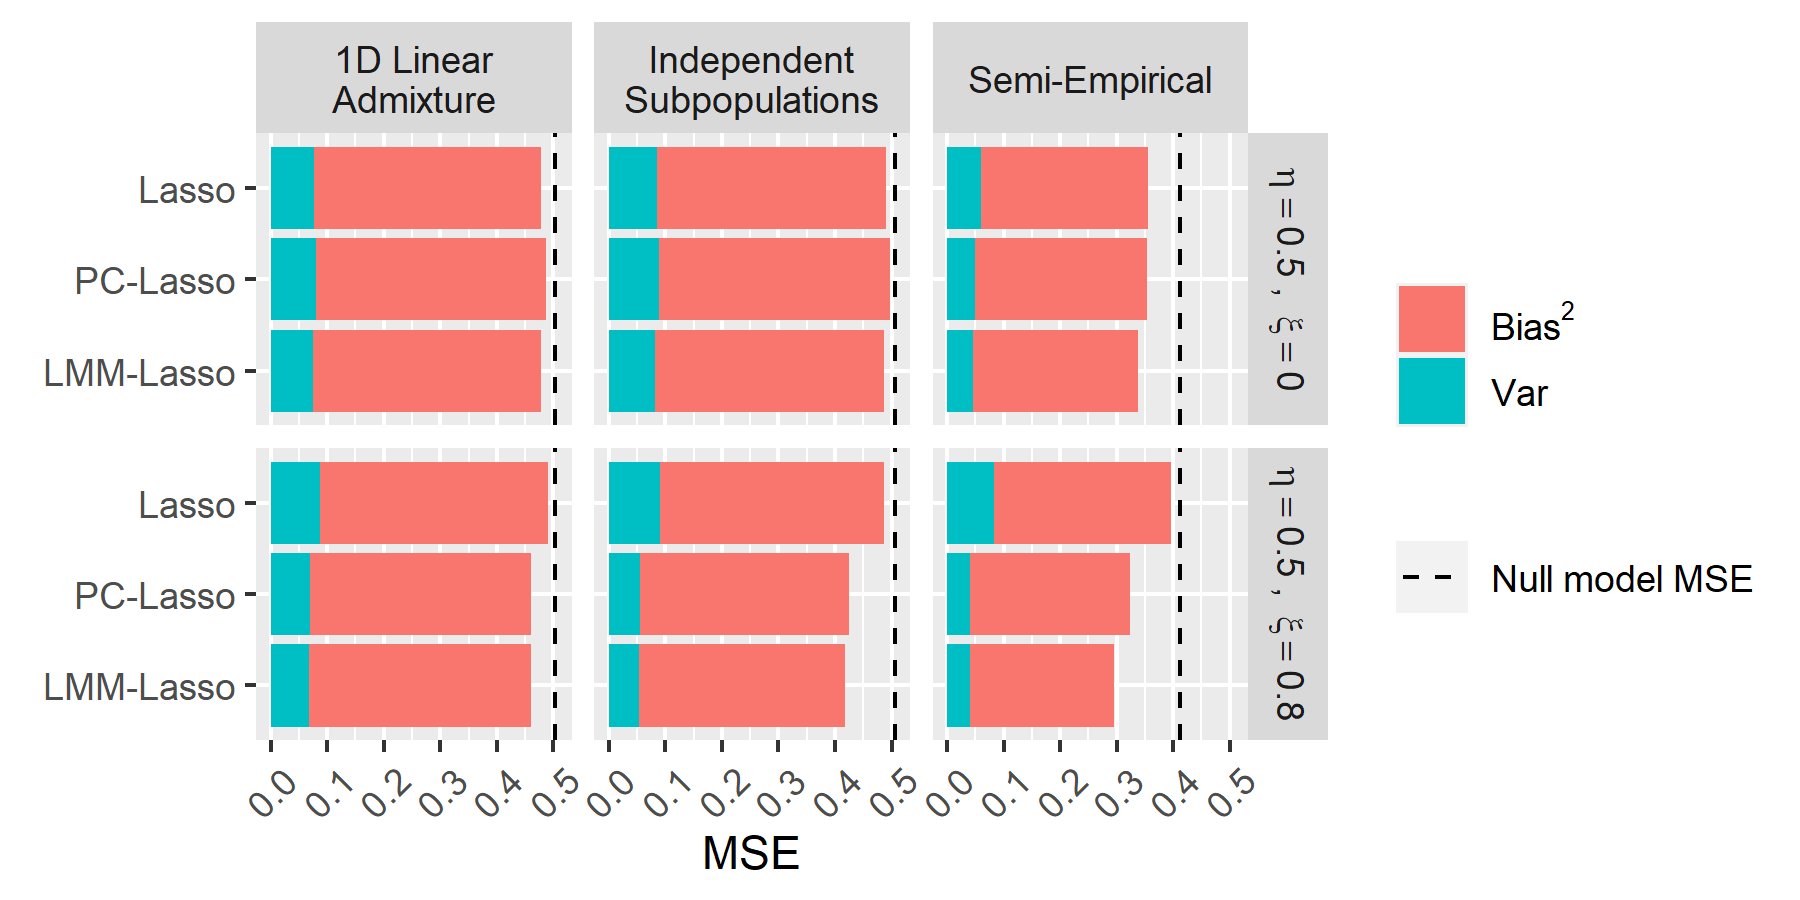
\includegraphics[width = \textwidth]{figures/beta_mse.png}
    \caption{Estimation accuracy of different methods for different data types in the presence and absence of environmental confounding with 4 subpopulations. Mean and 1 standard error (SE) bars displayed for 1000 replications.}
    \label{fig:mse}
\end{figure}

The bottom row of Figure \ref{fig:mse} shows the MSE when $\xi = 0.8$ (substantial environmental effects). In this case, both PC-lasso and LMM-lasso clearly outperform the ordinary lasso. This improvement is more substantial in the Empirical and Independent Subpopulations data than in the 1D Linear Admixture data. This is because there is less overlap between subpopulations than in the admixture data, meaning that a greater proportion of the environmental effect is in the column space of $\P_{\bX}$. We can quantify this proportion using the CP metric defined in \eqref{eqn:ratio}. Here, we have CP = 0.47, 0.87, and 0.99 for the 1D Linear Admixture, Empirical, and Independent Subpopulations, respectively. The large CP of the Empirical and Independent Subpopulations shows that the environmental effect is more highly correlated with genotype, and therefore has more potential for introducing bias into the estimation of SNP effects; the PC-lasso and LMM-lasso methods correct for this effect, while ordinary lasso does not.  This phenomenon occurs in 1D Linear Admixture setting as well, although the phenomenon is less pronounced because, while the total environmental effect is the same in all three settings, in the admixture setting 53\% of the environmental effect is uncorrelated with genotype and therefore does not introduce bias.

In addition to MSE, these methods' performance was also assessed in terms of variable selection using the true positive rate (TPR) for the first 50 variables each method allowed into the model. Throughout, we use ``true positive'' to mean both that the SNP was selected and that its direction was estimated correctly. Table \ref{tab:var_sel} displays the average TPR for the same settings as in Figure \ref{fig:mse}. The TPRs echo the MSE results in that lasso and LMM-lasso perform comparably in the absence of environmental confounding across all data types, with PC-lasso slightly less accurate at identifying causal SNPs. In the presence of environmental confounding, both LMM-lasso and PC-lasso achieve substantial improvements in TPR over the ordinary lasso. As with the MSE data, these improvements are more substantial in the Independent Subpopulations and Empirical data sets than in the 1D Linear Admixture data.

\begin{table}[H]
\centering
\begin{tabularx}{400pt}{cclYYY}
\toprule
$\eta$ & $\xi$ & \multicolumn{1}{c}{Method} & 1D Linear Admixture & Independent Subpopulations & Empirical \\ 
\midrule
\multirow{6}{*}{0.5} & \multirow{3}{*}{0} & lasso & 0.25 (0.05) & 0.23 (0.05) & 0.37 (0.06) \\ 
& & PC-lasso & 0.23 (0.05) & 0.21 (0.05) & 0.36 (0.06) \\ 
& & LMM-lasso & 0.25 (0.05) & 0.23 (0.05) & 0.41 (0.06) \\ 
\cmidrule{2-6}
& \multirow{3}{*}{0.8} & lasso & 0.24 (0.05) & 0.26 (0.06) & 0.29 (0.06) \\ 
& & PC-lasso & 0.28 (0.05) & 0.36 (0.06) & 0.46 (0.06) \\ 
& &  LMM-lasso & 0.28 (0.05) & 0.39 (0.06) & 0.61 (0.06) \\ 
\bottomrule
\end{tabularx}
\caption{True positive rates, defined as the proportion of the 50 causal SNPs which are selected with the correct sign, for different data types in the absence ($\xi = 0$) and presence ($\xi = 0.8$) of environmental effects. For the data sets with simulated genotypes, 4 subpopulations are present. Mean (SD) of 1000 replications.}
\label{tab:var_sel}
\end{table}

%------------------------------%
\subsection{PC-lasso and LMM-lasso reduce selection bias}
%------------------------------%

As described earlier in the manuscript, correlation between environmental effects and genotype introduces the potential to observe spurious associations in which SNPs that differ in frequency between subpopulations are identified as contributing to the phenotype.  In this section, we characterize the three lasso methods (ordinary, PC, and LMM) in terms of their susceptibility to this form of selection bias.

In order to assess the behavior of these methods in this context, we conducted a simulation using Empirical genotypes, but restricted to just two subpopulations, Caucasian and African-American.  A total of 1000 SNPs were chosen such that the selected SNPs' absolute difference in MAF between the two subpopulations ranged uniformly from 0 to 0.5. As in the earlier simulations, a 1:1 SNR ($\eta = 0.5$) was used to simulate the phenotype.

\begin{figure}[hbt]
\centering
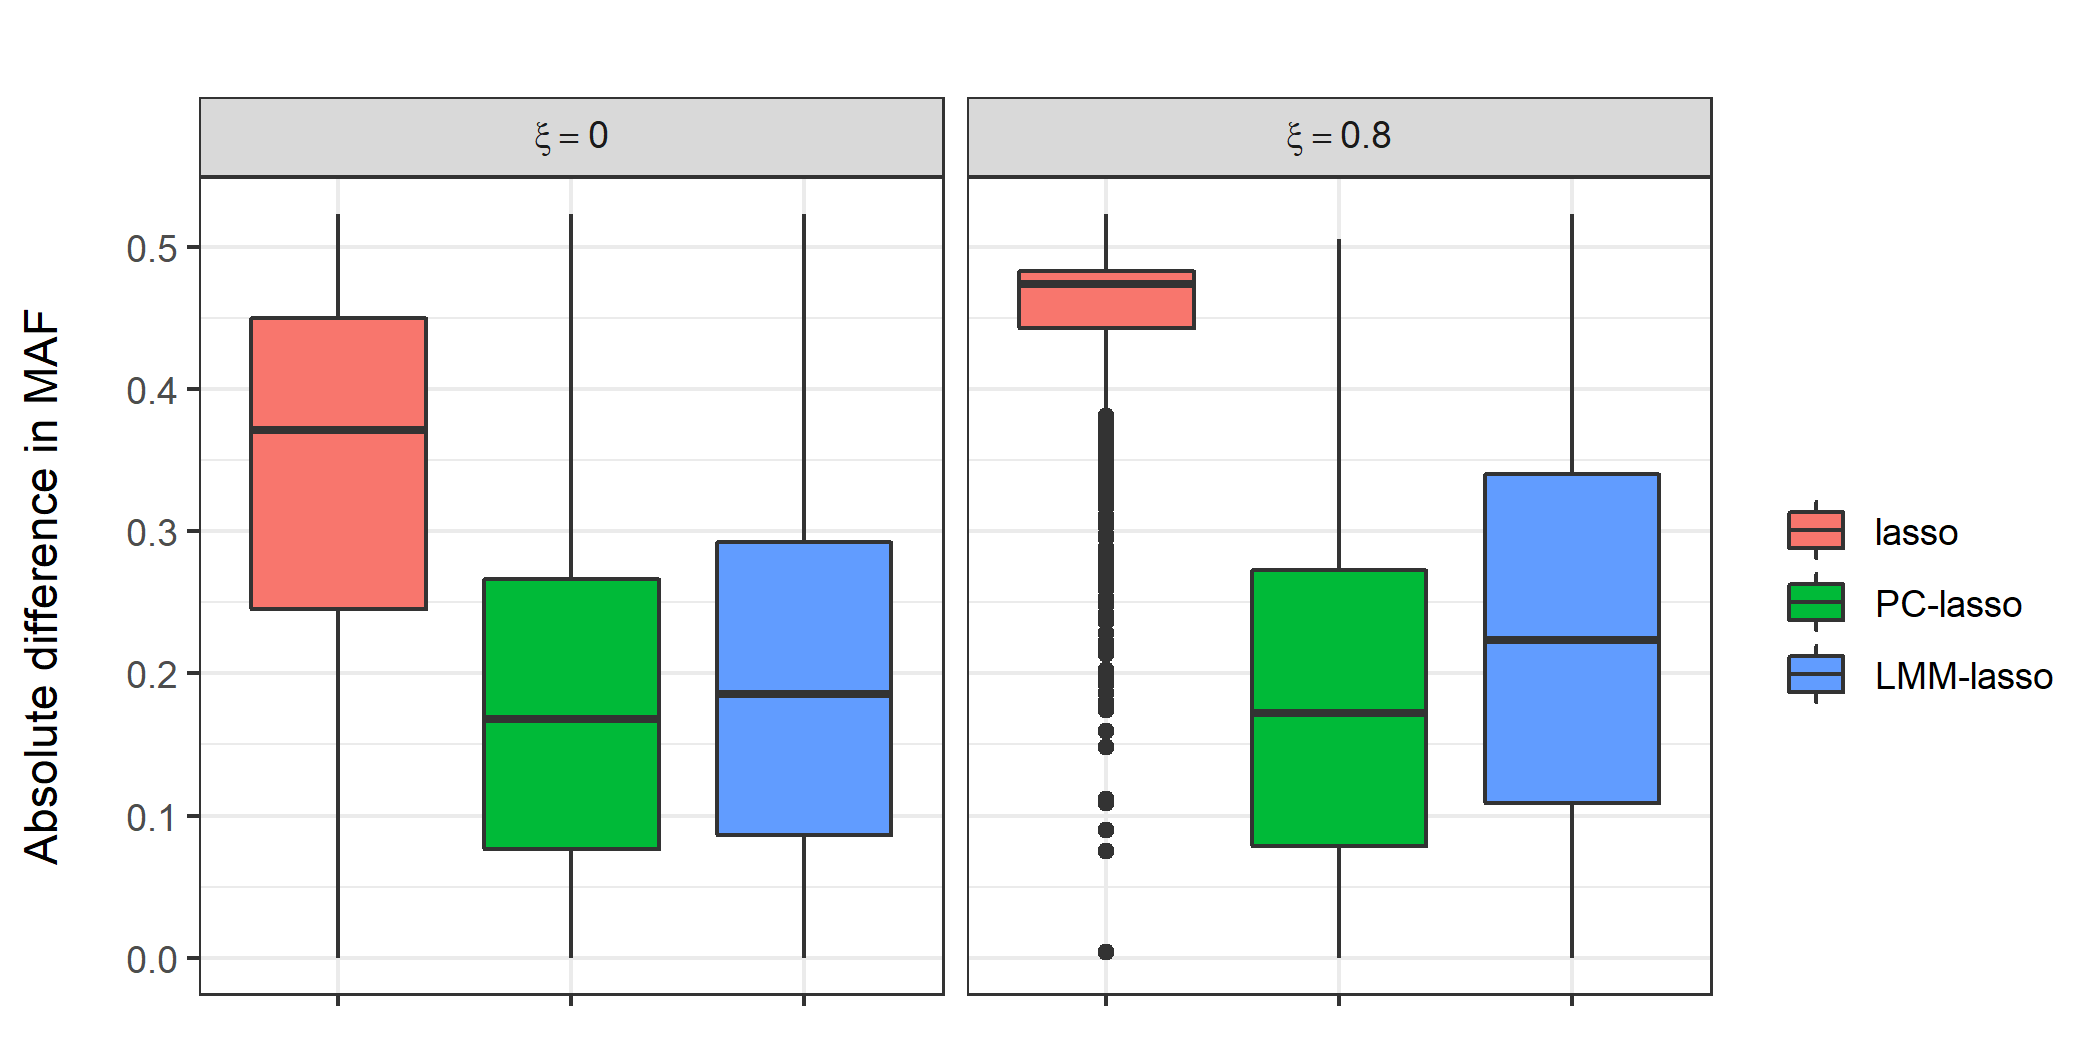
\includegraphics[scale = 0.9]{figures/pop_inf_snps_box.png}
\caption{Absolute allele frequency differences of selected, non-causal SNPs across methods, in the presence and absence of environmental confounding for two Empirical subpopulations, $\eta = 0.5$, 1000 replications.}
\label{fig:pop_inf}
\end{figure}

Figure \ref{fig:pop_inf} summarizes each method's tendency to select spurious associations driven by differences in MAF between populations.  Even in the absence of environmental effects, the ordinary lasso shows a preference for selecting population-informative SNPs, while PC-lasso and LMM-lasso are reluctant to select such SNPs (recall that with this design, the median MAF difference between populations is 0.25).  In the presence of confounding, however, the lasso shows an overwhelming tendency to select population-informative SNPs.  Its false positive selections are almost always the ones with the largest differences between populations.  PC-lasso and LMM-lasso, on the other, show no such such selection bias.


%------------------------------%
\subsection{LMM-lasso outperforms PC-lasso for finer population structures}
\label{sec:sim-fine-coarse}
%------------------------------%

Although PC-lasso and LMM-lasso outperform the ordinary lasso in the presence of environmental confounding, they are not equally effective across all population structures.  Here, we compare the performance of these two methods in two settings, as described in Section~\ref{sec:subpopulation_structure}: ``coarse'' (4 subpopulations) and ``fine'' (100 subpopulations).  Synthetic phenotypes were simulated using a 1:1 SNR ($\eta = 0.5$) and varying levels of environmental confounding, $\xi \in \{0.2, 0.5,0.8\}$. 

\begin{figure}[H]
    \centering
    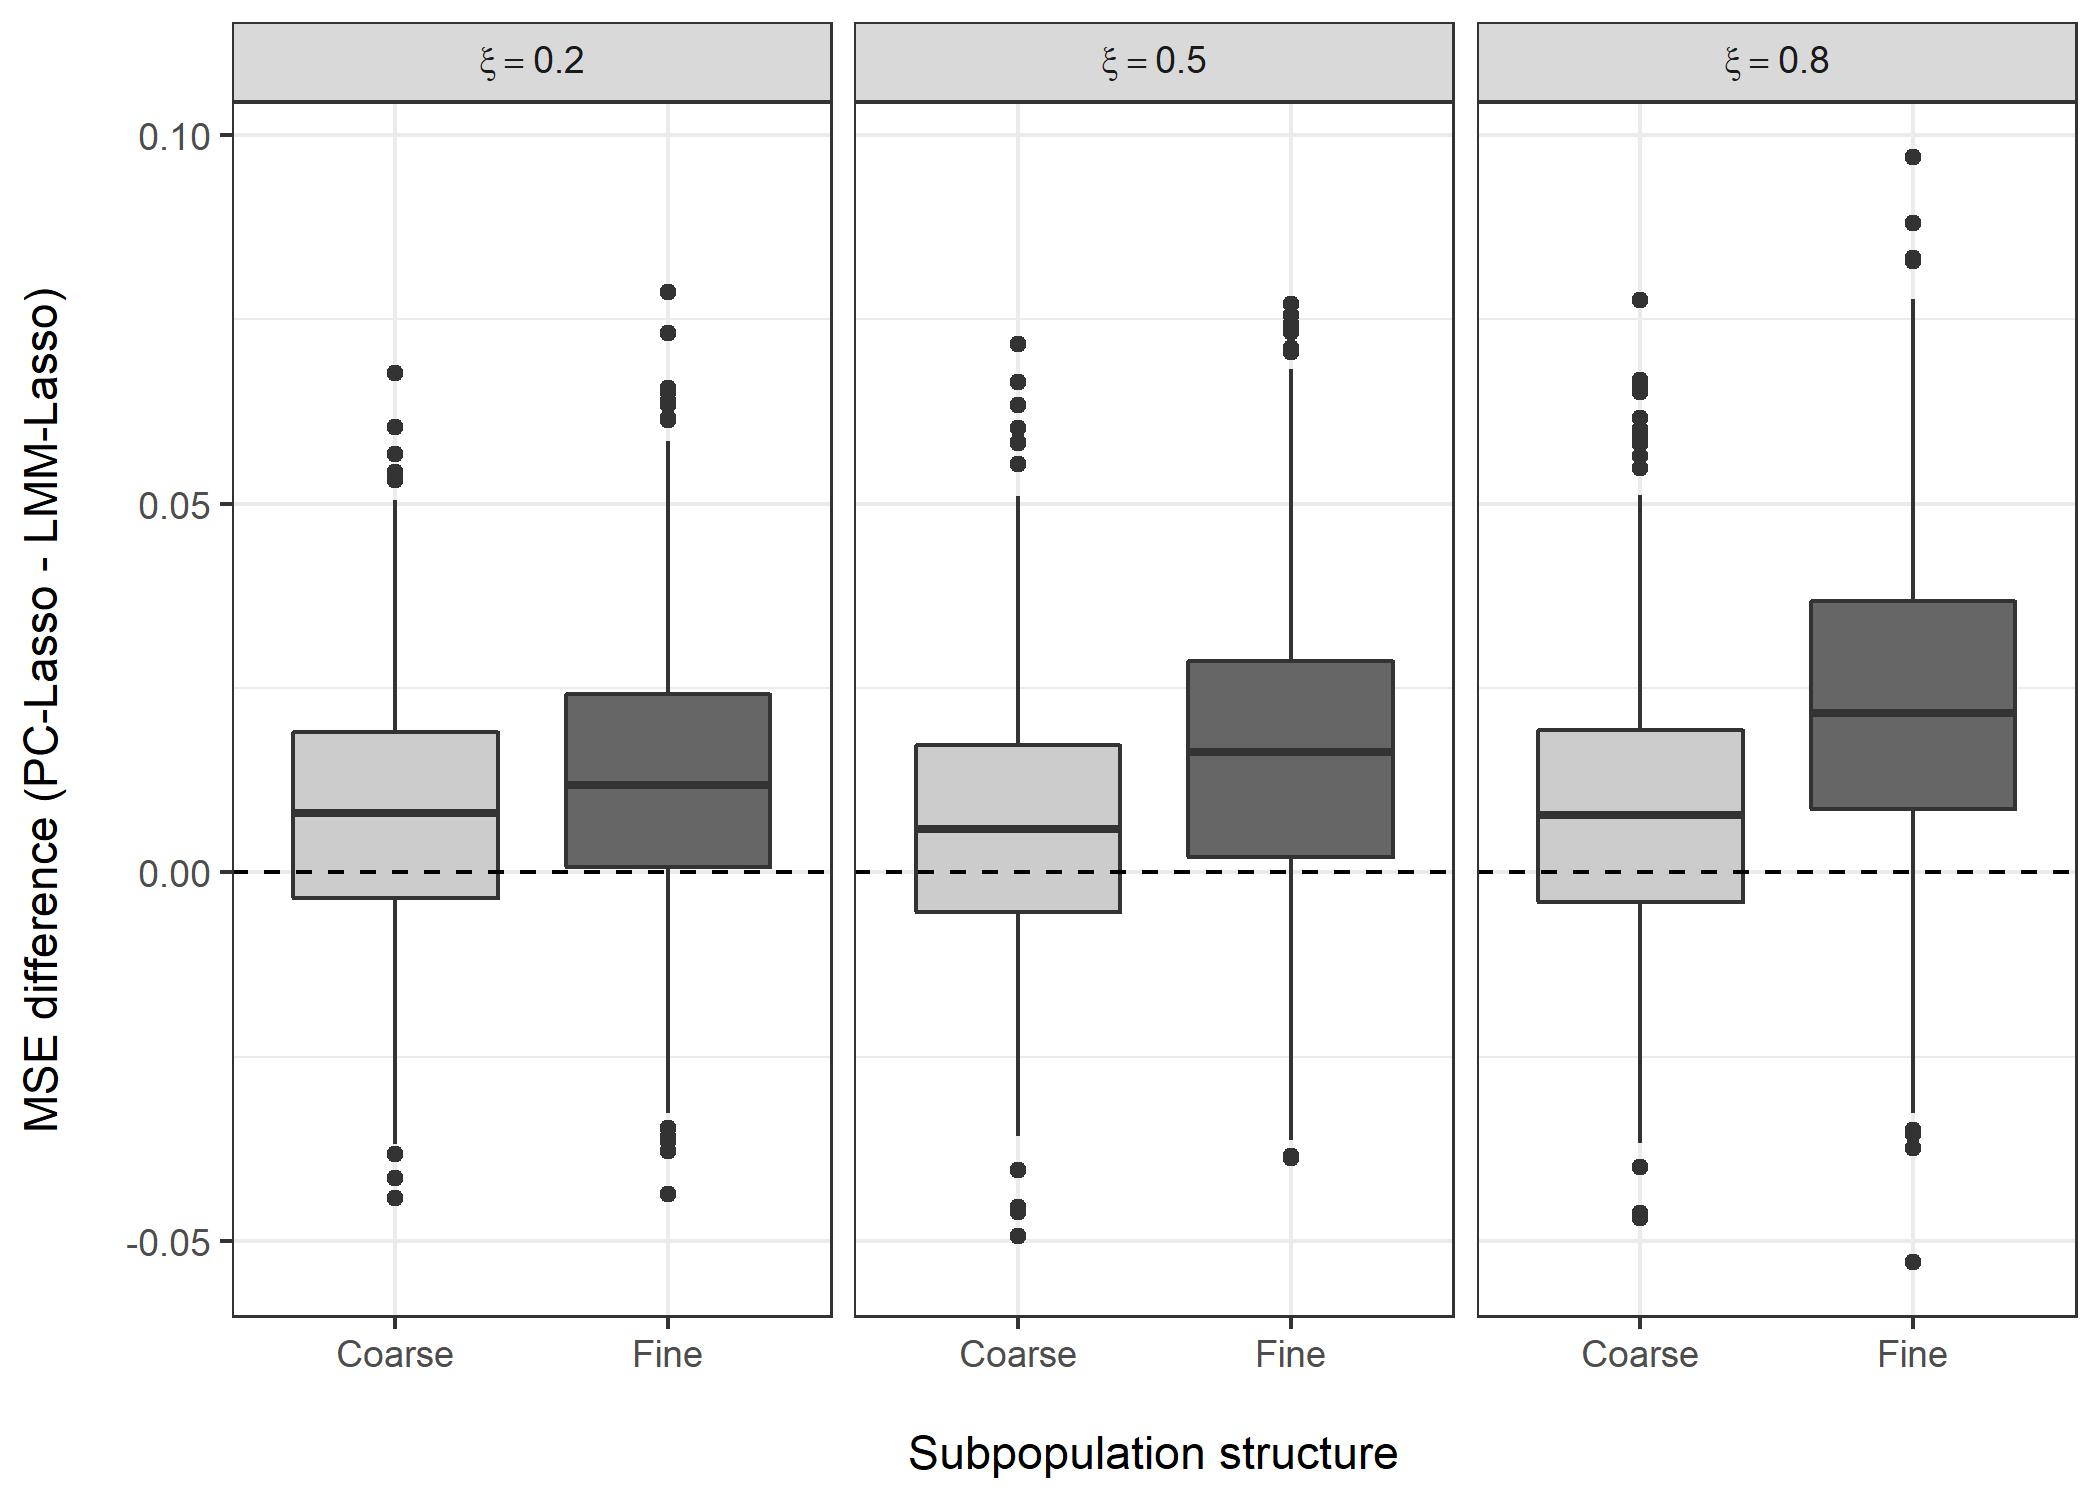
\includegraphics[scale = 0.9]{figures/mse_diff_subpops.png}
    \caption{Relative performance of LMM-lasso, PC-lasso for fine and coarse subpopulation structures and varying levels of environmental confounding with Independent Subpopulations, $\eta = 0.5$, 1000 replications.}
    \label{fig:big_vs_small}
\end{figure}

Figure \ref{fig:big_vs_small} summarizes the results of these simulations. The vertical axis displays the difference in MSE: PC-lasso $-$ LMM-lasso, so that positive numbers correspond to LMM-lasso outperforming PC-lasso and vice versa. The dashed horizontal line at 0 indicates no difference in the performance the two methods.

In all settings, LMM-lasso outperformed PC-lasso, although the difference was considerably more pronounced when the subpopulation structure was fine.  These findings are consistent with \citet{hoffman2013correcting}, who showed that PC adjustment methods represent a low dimensional approximation to LMMs. As such, it is reasonable that PC-lasso, which corrects for population structure using a low dimensional set of surrogate variables, would perform reasonably well in settings with coarse population structures, but fall short when the structure is more complex.

%------------------------------%
\subsection{Implementations of LMM-lasso}
%------------------------------%

In Section \ref{sec:lmmlasso} we briefly mentioned the existence of two LMM-lasso variants: LMM-lasso-Rakitsch and LMM-lasso-ggmix. Both methods perform quite similarly in terms of estimation and variable selection for the settings presented in Sections~\ref{sec:sim-mse}-\ref{sec:sim-fine-coarse}. Because of this, the preceding results, though generated using the LMM-lasso-Rakitsch implementation, are representative of both LMM-lasso methods in the $n = 200, p = 1000$ setting. The primary purpose of this review is to compare LMM-lasso to other penalized regression methods with respect to correcting for population structure and environmental confounding. However, given the generally strong performance of LMM-lasso, in this section we describe the key differences between these two implementations and provide guidance for potential users.

LMM-lasso-Rakitsch uses a two-step approach. First, the variance components are estimated under the assumption of a null model. Then, the estimated variance components are used to transform the data, and $\bbeta$ is estimated using coordinate descent. LMM-lasso-ggmix seeks to improve upon this procedure by re-estimating the variance components and $\bbeta$ iteratively. Although this seems a reasonable idea, our experiments reveal that it makes little to no difference in terms of estimating $\bbeta$. In order to systematically compare both methods, we carried out simulations where $p = 1000$, $n = \{200, 400, 600, 800, 1000, 1200, 1400\}$, and $\eta = \{0.2, 0.5, 0.8\}$. Figure \ref{fig:eta_beta_mse} shows the MSE for estimation of $\bbeta$ and $\eta$, in addition to the corresponding computing time required. 

LMM-lasso-Rakitsch and LMM-lasso-ggmix achieve nearly identical MSE for $\bbeta$ in almost all scenarios, particularly when $n \ll p$ (Figure \ref{fig:eta_beta_mse}, top panel). However, when $n \ge p$ the estimation performance of LMM-ggmix becomes erratic, occasionally far worse than that of LMM-lasso-Rakitsch. This is most dramatic in the presence of substantial environmental environmental confounding, $\xi = 0.8$, and $n = \{1200, 1400\}$. 

LMM-lasso-ggmix does tend to provide improved estimates of $\eta$ compared to LMM-lasso-Rakitsch, particularly in the presence of lower $\eta$ values and where $n \ll p$ (Figure \ref{fig:eta_beta_mse}, middle panel), although these improvements did not help it to estimate $\bbeta$ more accurately. In addition, at high signal-to-noise ratios ($\eta=0.8$), the performance of LMM-lasso-ggmix was highly variable.

Overall these results show that LMM-lasso-ggmix performs similarly to LMM-lasso-Rakitsch in estimating $\bbeta$ and outperforms LMM-lasso-Rakitsch in estimating $\eta$ when $n \ll p$. However, these are also the settings in which LMM-lasso-ggmix is least computationally efficient. The bottom panel of Figure \ref{fig:eta_beta_mse} shows the computing time required of each method in the various simulation settings, and shows that when $n \ll p$, LMM-lasso-ggmix is up to 60 times slower than LMM-lasso-Rakitsch. In settings where $n \ge p$, LMM-lasso-ggmix is ``faster'' than LMM-lasso-Rakitsch, but this seems to be due to the algorithm getting stuck in a local minimum and prematurely terminating, a phenomenon that also explains the extremely poor estimation accuracy of LMM-lasso-ggmix in the $\eta=0.8$, $n=1400$ setting.

The underlying reason for this is that the RRM becomes ill-conditioned when $n > p$ \citep{ledoit2004well}. Although both approaches utilize the RRM, because LMM-lasso-ggmix attempts to estimate more parameters than LMM-lasso-Rakitsch, its optimization problem is no longer convex, making it prone to becoming stuck in local minima before it is able to sufficiently explore the coefficient path. This phenomenon is illustrated in greater detail in Supplementary Figure \ref{fig:niter}.

\begin{figure}[H]
    \centering
    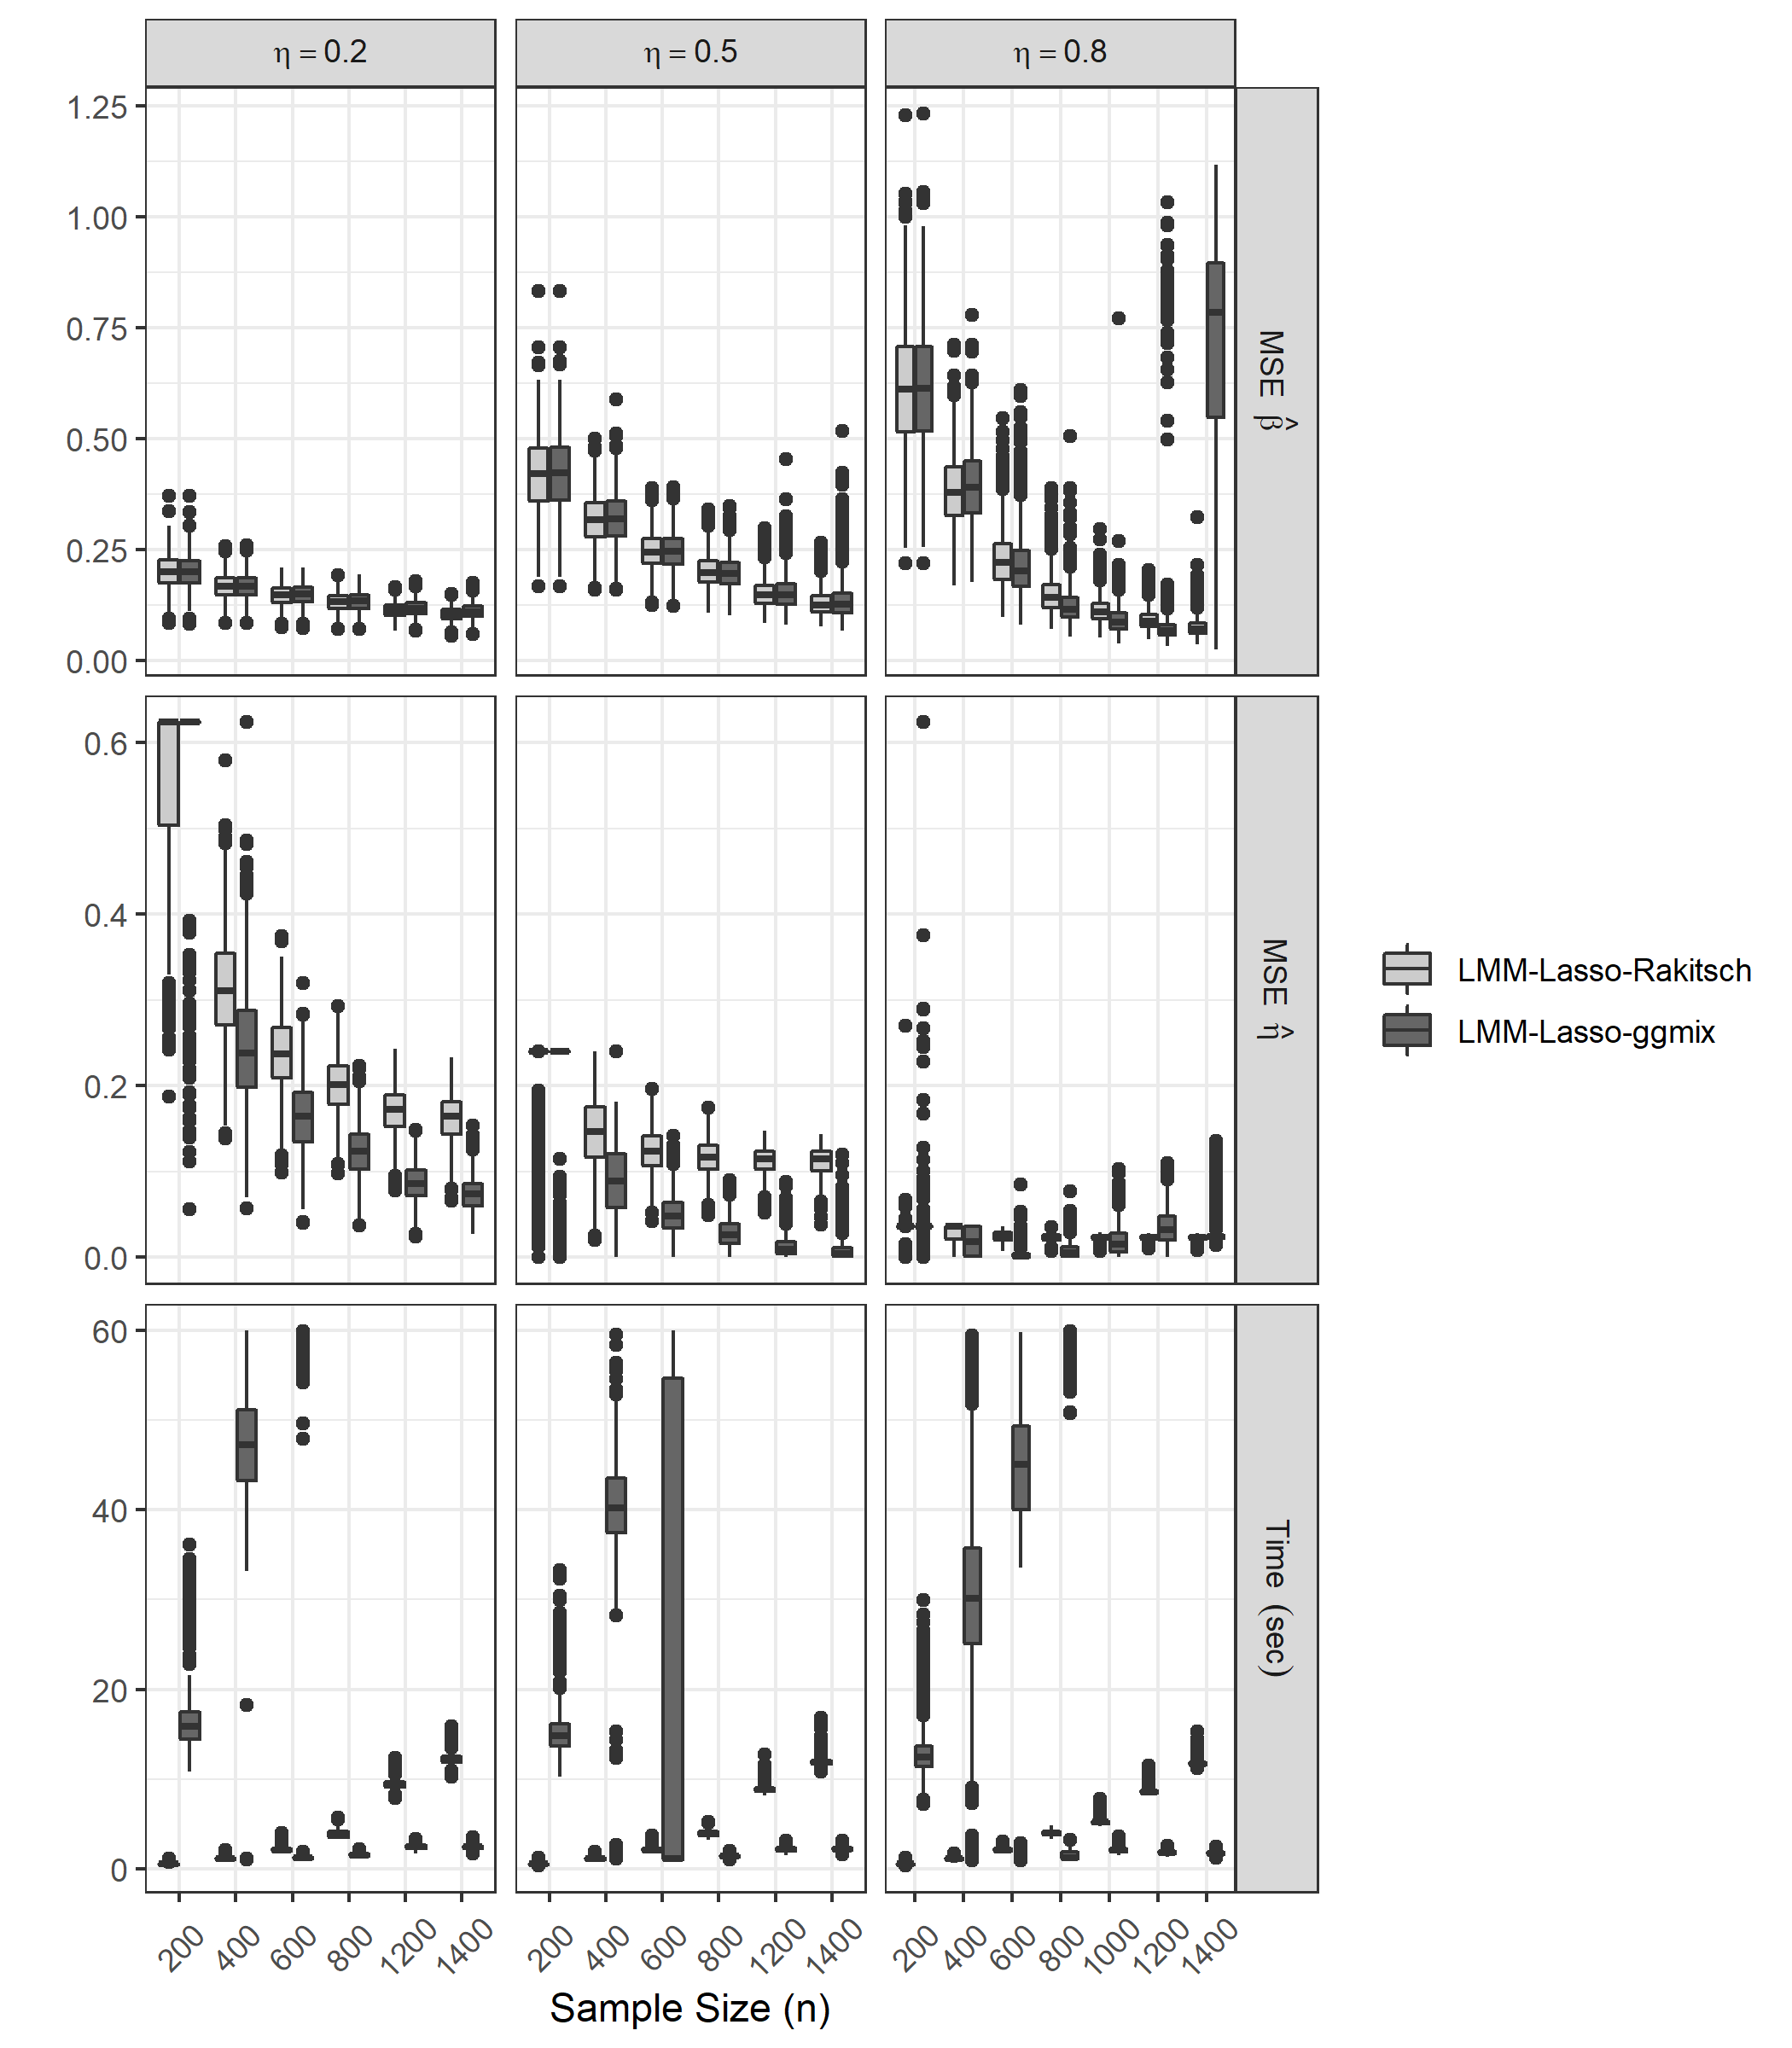
\includegraphics[width = \textwidth]{figures/eta_beta_hat.png}
     \caption{Estimation accuracy and computing time of LMM-lasso-Rakitsch and LMM-lasso-ggmix for $\bbeta$ and $\eta$ for varying $\eta$ levels and sample sizes with Independent Subpopulations data, coarse subpopulation structure, $\xi = 0.8$, 1000 replications.}
    \label{fig:eta_beta_mse}
\end{figure}

%------------------------------%
\subsection{\anna{Genome-wide analysis case study}}
%------------------------------%

\begin{figure}[hbt]
\centering
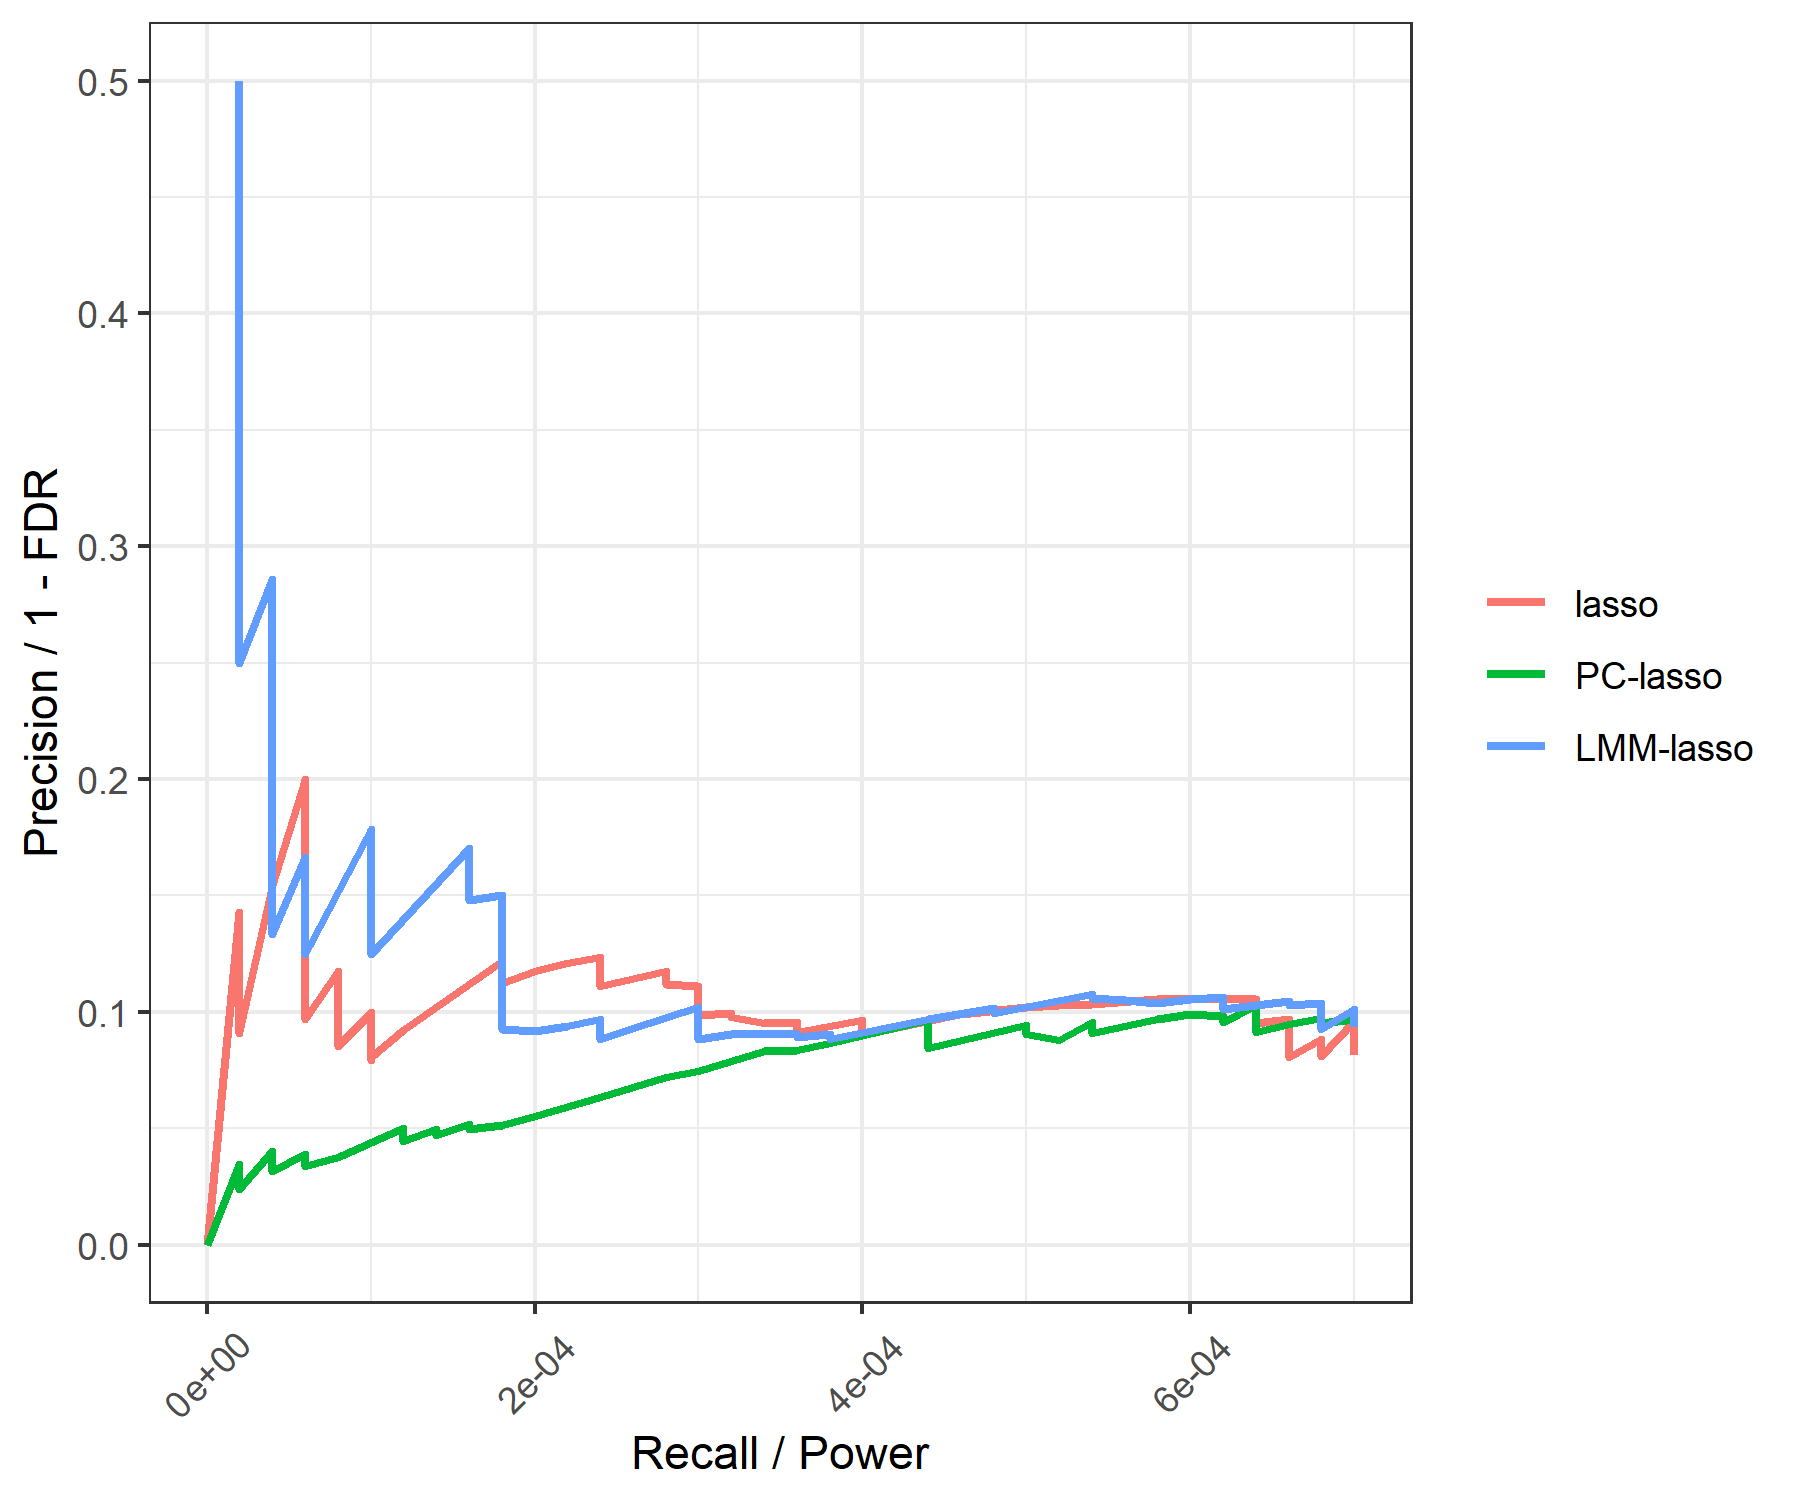
\includegraphics[scale = 0.9]{figures/genomewide_prc.png}
\caption{Precision recall curves across $\lambda$ values from the Empirical genome-wide analysis. Single replication case study with $\eta = 0.5, \xi = 0.8$.}
\label{fig:gw_prc}
\end{figure}

\begin{figure}[hbt]
\centering
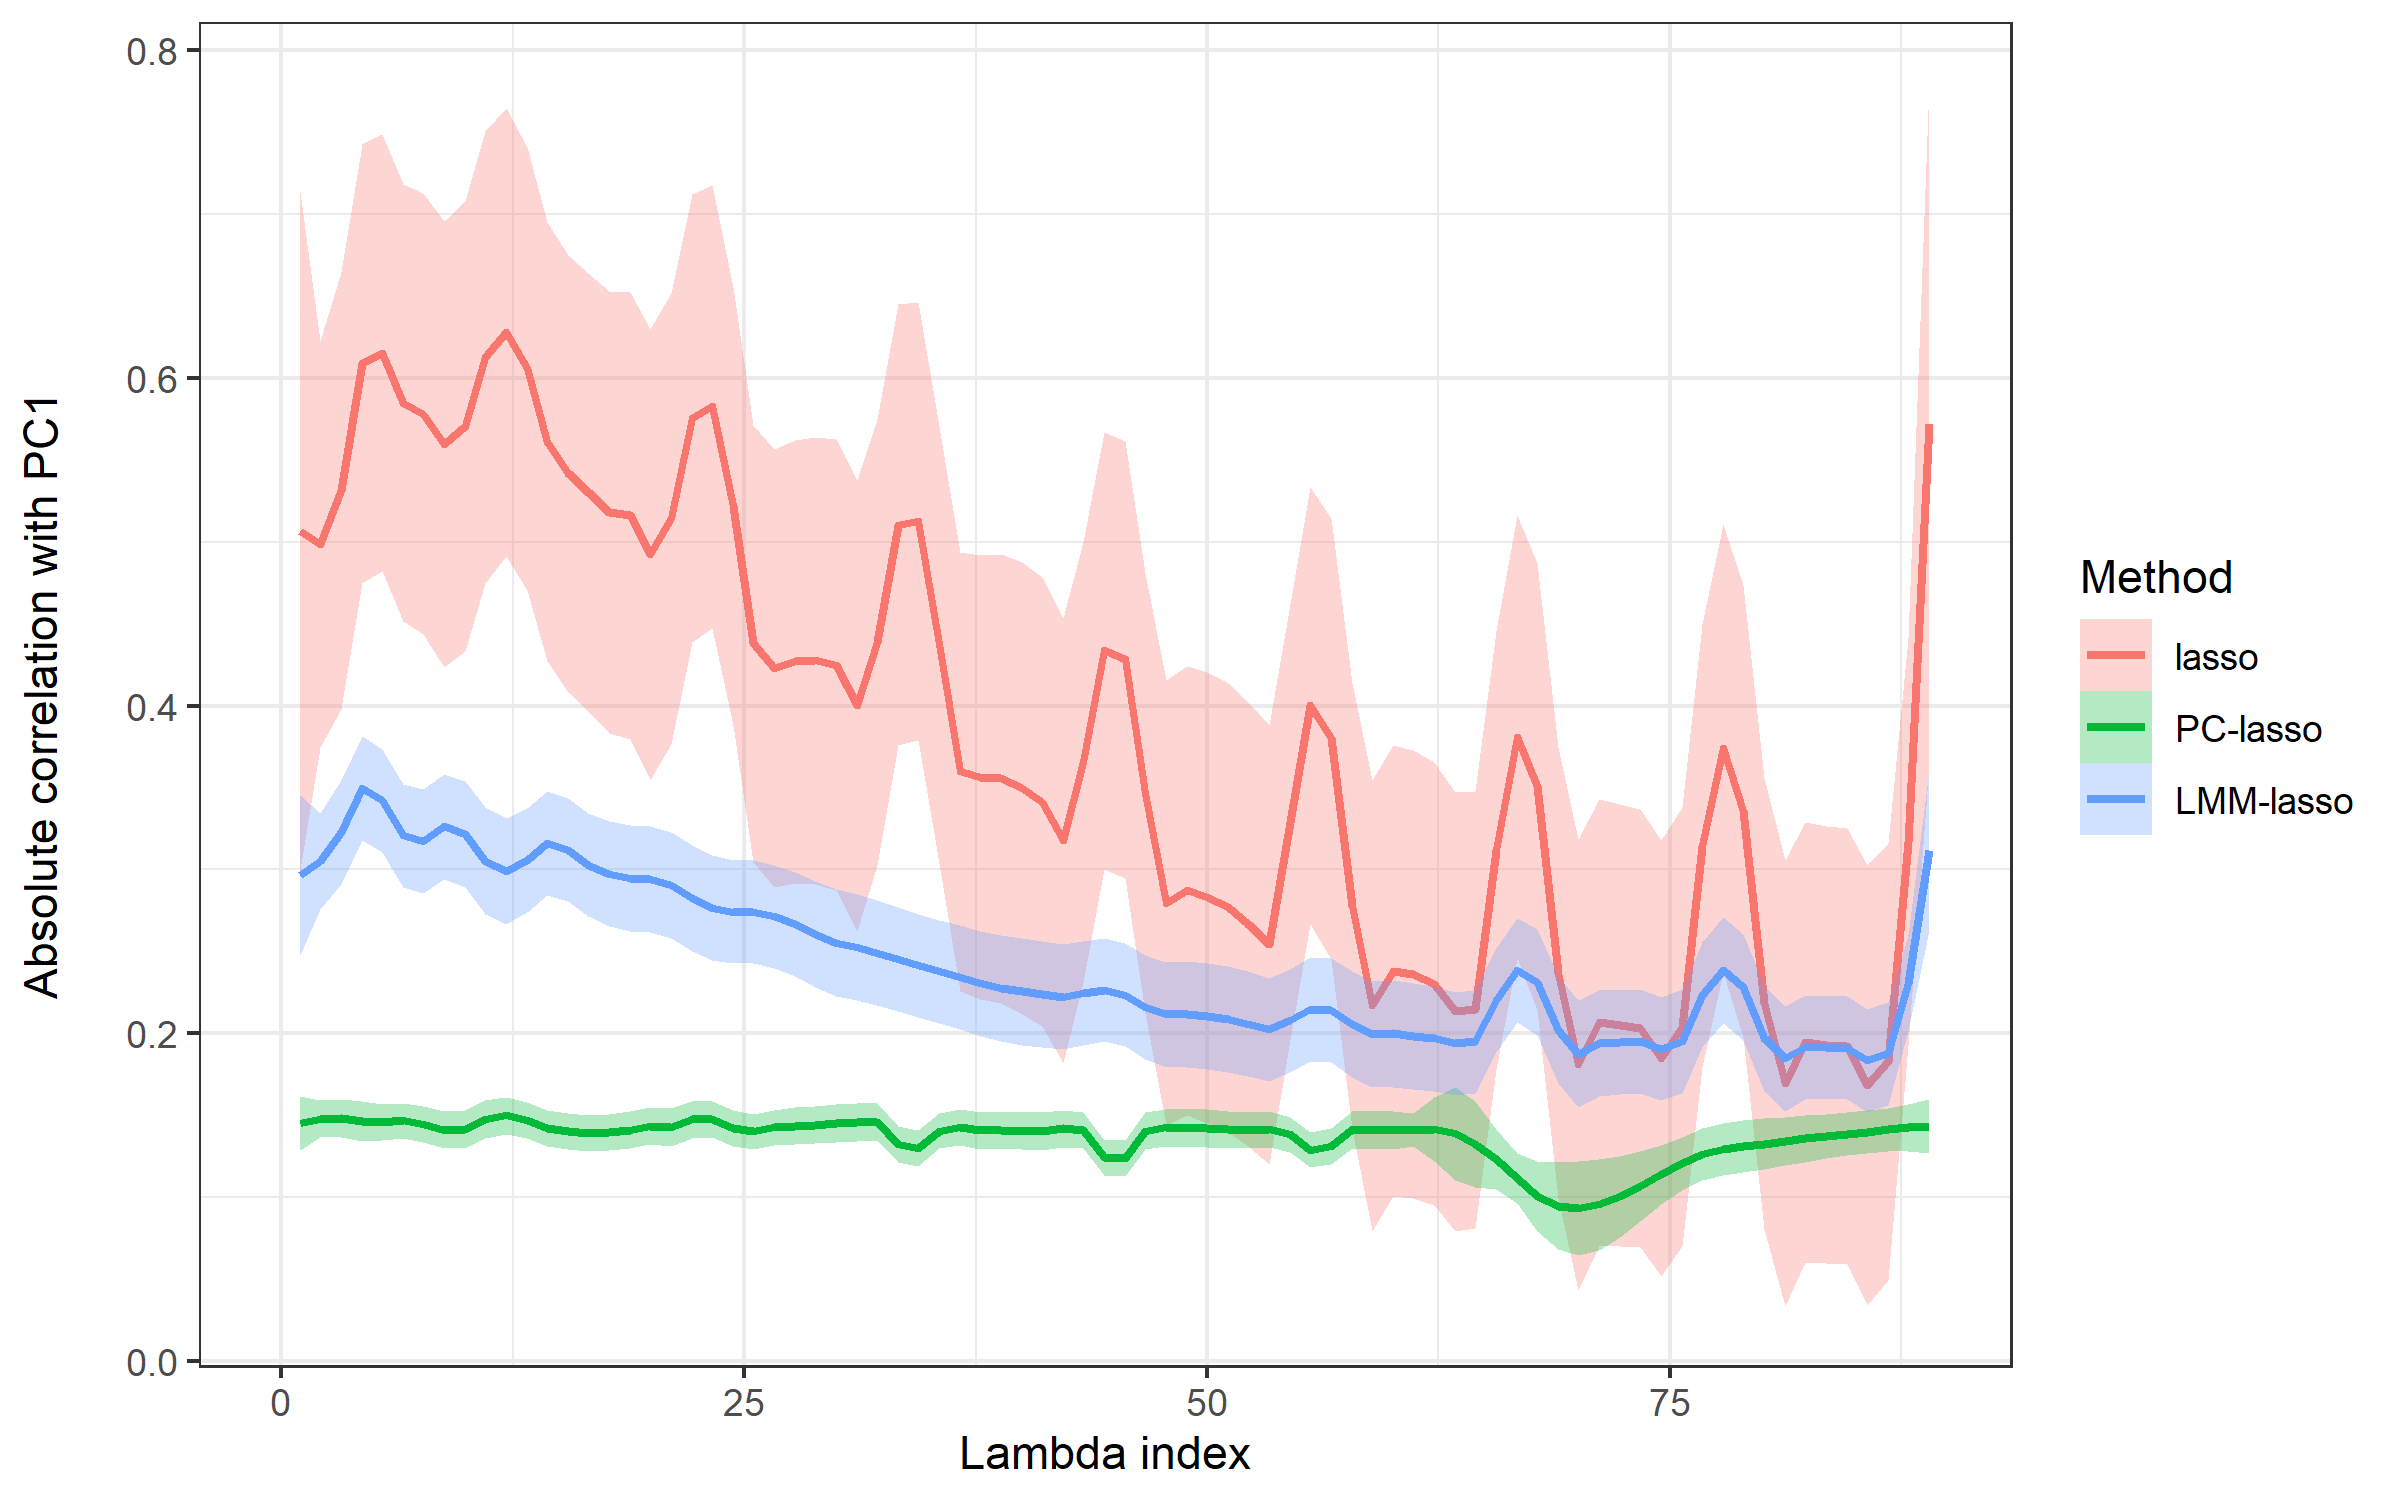
\includegraphics[scale = 0.9]{figures/genomewide_pc1_corr.png}
\caption{Pathwise absolute correlation of selected, non-causal SNPs with the first principal component of the data in Empirical genome-wide analysis. Plotted line is the mean absolute correlation of all incorrectly selected SNPs for a particular $\lambda$ value, with shaded region for $\pm$ 1 SE. Single replication case study with $\eta = 0.5, \xi = 0.8$.}
\label{fig:gw_pc1_corr}
\end{figure}

%%%%%%%%%%%%%%%%%%%%%%%%%%%%%%%%
%------------------------------%
%%%%%%%%%%%%%%%%%%%%%%%%%%%%%%%%
\section{Discussion} \label{sec:discussion}
%%%%%%%%%%%%%%%%%%%%%%%%%%%%%%%%
%------------------------------%
%%%%%%%%%%%%%%%%%%%%%%%%%%%%%%%%

In this work, we reviewed the concept of population structure in a framework which formally differentiates between effects of population structure and those of the environment. We have provided a broad outline of existing  methods for ameliorating the effects of these unobserved confounding influences. In addition, we have provided a thorough review of two penalized regression approaches that correct for population structure in genetic data: PC-lasso and LMM-lasso. We have detailed the assumptions made by PC-lasso and LMM-lasso, which model confounding influences as fixed and random effects, respectively. We have also described the ways in which prior analyses of these methods may fail to accurately capture the effects of environmental effects in terms of contributing to selection and estimation bias. We hope that our result partitioning environmental effects into confounding and non-confounded components will be particularly useful in terms of understanding the performance of these approaches.

Our simulations experiments reveal, unsurprisingly, that PC-lasso and LMM-lasso outperform the ordinary lasso whenever environmental confounding effects are present. However, in the absence of such effects, PC-lasso may hinder estimation accuracy. Additionally, we find that LMM-lasso consistently outperforms PC-lasso, especially when the population structure is more complex. These results indicate that LMM-lasso is a more robust method in practice when the nature of the population structure is unknown.

We considered two implementations of the LMM-lasso method: LMM-lasso-Rakitsch and LMM-lasso-ggmix, which differ in their variance estimation procedures and computational implementations. Although both methods perform similarly in terms of estimating $\bbeta$, the much greater computational efficiency and numerical stability of LMM-lasso-Rakitsch make it a more attractive choice in most scenarios, although LMM-lasso-ggmix may be useful if the objective of the analysis is to accurately estimate variance components.

Although the purpose of this article is to elucidate the manner in which failing to correct for unobserved environmental effects can bias SNP effect estimates, equation \eqref{eqn:partition_e} also highlights the manner in which such unobserved environmental effects can lead to substantial bias in narrow-sense heritability estimates using SNP data. In particular, these estimates are likely to be inflated by the quantity $\boldsymbol{\tau}$ unless steps are taken to address population structure. A detailed treatment of narrow-sense heritability estimation is beyond the scope of this paper, but we hope this emphasizes the broad implications and importance of distinguishing between population structure and environmental effects.

\anna{The nature of the simulations and analyses in this work have allowed us to select penalty parameters based on the true number of causal features in a model, which allows for fair comparison across methods. In a real data scenario, the true number of causal SNPs would not be known a priori. As such, appropriate methods for penalty parameter selection in penalized LMMs are worth additional discussion. As of yet there is no clear consensus on the optimal way to select a penalty parameter for penalized LMMs.}

\anna{Several authors have used the Bayesian information criterion (BIC) for variable selection in mixed models \cite{bondell2010joint, schelldorfer2011estimation}. However it has been shown that the Akaike information criterion (AIC) and BIC may perform poorly in the high-dimensional setting \citep{fan2013tuning}. The high-dimensional BIC introduced by \citet{fan2013tuning} penalizes model parameters more severely in an attempt to perform better in high dimensional settings. \citet{bhatnagar2020simultaneous} employs this high-dimensional BIC as its default method to select $\lambda$.}

\anna{Subsampling approaches, such as CV and stability selection, are another common class of variable selection methods often preferred to information criterion-based approaches. \citet{rakitsch2013lasso} used stability selection to evaluate the significance of individual SNPs \citep{meinshausen2010stability}. \citet{guo2019combining} used a combination of both methods for feature selection, first selecting several $\lambda$ values via CV, and then using these penalty parameters for stability selection and final feature selection. As previously mentioned, however, the advisability of subsampling methods in the presence of correlated observations remains an open question \citep{roberts2017cross, jia2012preconditioning}. A rigorous assessment of penalty parameter selection in the context of penalized LMMs is beyond the scope of this work, but worthy of further investigation.}

\anna{\textbf{I don't think we should bring up the idea of CV/subsampling on original vs transformed data in this paper at all - I think it would just make things more confusing without a lot of additional explanation.}}

Finally, we note that this article has focused entirely on the lasso as a penalization scheme. This is reasonable, as it is the most widely used method. However, many other penalized regression approaches have been developed that aim to reduce bias, better account for correlation between features, and to account for the grouping of SNPs into genes. All of these approaches are potentially attractive avenues for future research into GWAS methodology.

\subsection*{Data Availability}

Data sharing is not applicable to this article as no new data were collected or analyzed in this study.
